\documentclass[a4paper,10pt]{article}
\usepackage[top=1in,bottom=1in,left=1in,right=1in]{geometry}
\usepackage{fullpage}
\usepackage[english,swedish]{babel}
\usepackage[T1]{fontenc} 
\usepackage[utf8]{inputenc}
\usepackage{amsmath}
\usepackage{amssymb}
\usepackage{amsthm}
\usepackage{amsfonts}
\usepackage[pdftex]{graphicx}
\usepackage{fancyvrb}
\usepackage{array}
\usepackage{fancyhdr}
\usepackage{courier}
\usepackage{booktabs}
\usepackage{paralist}
\usepackage{xfrac}
\usepackage{siunitx} % Provides the \SI{}{} and \si{} command for typesetting SI units
\usepackage{graphicx} % Required for the inclusion of images
\usepackage{amsmath} % Required for some math elements 
\usepackage{tikz}
\usetikzlibrary{arrows.meta}
% \usepackage{cite}
\usepackage{enumitem}
\usepackage{float}
\usepackage{wrapfig}
\usepackage{multicol}
\usepackage{caption}
\usepackage{svg}
% \usepackage{subcaption}
% \usepackage{natbib}
\usepackage[citestyle=verbose-ibid,bibstyle=numeric,backend=bibtex,sorting=nty]{biblatex}
\addbibresource{reference.bib}
\usepackage{csquotes}
\usepackage{pdfpages}
\usepackage{appendix}
\usepackage{url}
\usetikzlibrary{scopes}

\setlength\parindent{0pt}
\urlstyle{same}


\bibliography{sample}


% \let\oldtabular\tabular 
% \renewcommand{\tabular}{2pt}

% Ger en titelsida för bilagor
\renewcommand*{\appendixpagename}{\newpage Bilagor} 
\renewcommand*{\appendixtocname}{Bilagor} 

% Gör titel
\usepackage{titlesec}
% \titleformat{\section}{\normalfont\Large\bfseries}{\S \thesection}{1em}{}
\title{\Huge\bf{The application of Neural Networks for note recognition}\\}
\author{\emph{Niklas Gustin, Victor Sellstedt, Björn Thorén, Kristoffer Åhgren}\\Handledare: \emph{Lars Gråsjö}}
\date{2016-01-29}
\pagenumbering{gobble}


\begin{document}
\pagenumbering{gobble}
\null  % Empty line
\nointerlineskip  % No skip for prev line
\vfill
\let\snewpage \newpage
\let\newpage \relax
\maketitle
\let \newpage \snewpage
\vfill 
\break % page break


% \maketitle
% \newpage

% \section*{FÖRORD}
% Att skriva förord är inte obligatoriskt, men här har du utrymme att skriva en inledande text av mer personlig karaktär. Förordet ska vara mycket kortfattat (högst en halv sida) och beskriva arbetets tillkomst som inte berör det detaljerade innehållet. Ett förord kan bland annat beskriva:\\
% •	Namn på skolan, programmet etc.\\
% •	Utbildningens omfattning\\
% •	Gymnasiearbetets omfattning\\
% •	Medverkande företag\\
% •	Tack till namngivna personer som varit behjälpliga med arbetet\\
% Observera att förordet inte har någon kapitelnumrering. 

\selectlanguage{english}
\begin{abstract}{}

Research of neural networks is essential for the continued development of modern artificial intelligence and deep learning structures. Neural networks are very useful tools to identify patterns, such as face recognition, that might be simple for humans to recognize but difficult for computers. With the seemingly endless possibilities for neural networks it raises the question of what is required for a neural network to be able to differentiate between different musical tones. By creating our own neural network and using generated data we studied the results generated by networks distinguishable by number of layers and nodes when they were given real, recorded tones. The results showed that differentiating between all of the tones of a smaller piano is a too complicated task for a three layer network to complete. By adding layers and nodes while reducing the number of tones to distinguish, we managed to create networks that were more sucessfull. Further research must be made, but this implies that by adding layers and nodes it might be possible to identify all of the tones, but at the cost of longer training time.

% Sammanfattningen ska spegla hela rapportens innehåll i huvudkomponenterna Syfte, Metod, Resultat och Slutsatser. Detta innebär att du berättar kort om vad arbetet gick ut på, vad syftet var, tillvägagångssättet d v s hur arbetet genomfördes, vilka resultat som kom fram samt vilka slutsatser som dragits. Man får här inte tillföra något nytt som inte har skrivit om inne i själva rapporten och omfattningen bör vara 100–150 ord. Sammandraget skrivs löpande i ett enda stycke på engelska. Sammandraget skrivs när resten av uppsatsen är klar. 

% Observera att sammanfattningen på engelska inte har någon kapitelnumrering. 
\end{abstract}
\selectlanguage{swedish}
\newpage
\tableofcontents
\pagenumbering{arabic}
% INNEHÅLLSFÖRTECKNING
% FÖRKORTNINGAR OCH BEGREPP	1
% 1. INLEDNING	2
% 1.1 BAKGRUND	2
% 1.2 TEORI	2
% 1.2.1 Rubrik nivå 3	3
% 1.3 SYFTE OCH FRÅGESTÄLLNINGAR	2
% 1.4 AVGRÄNSNINGAR	2
% 1.5 RAPPORTENS DISPOSITION (EVENTUELLT)	2
% 2. METOD	3
% 3. RESULTAT	4
% 4. DISKUSSION	5
% 4.1 TOLKNING AV RESULTAT	5
% 4.2 METODANALYS	5
% 4.3 BEDÖMNING AV METODENS GILTIGHET	5
% 4.4 REFLETION ÖVER ARBETET	5
% 4.5 FRAMTID	5
% REFERENSLISTA	6
% BILAGOR	7
\newpage
\section{FÖRKORTNINGAR OCH BEGREPP}

\begin{enumerate}[noitemsep]
\item NN - Neurala nätverk
\item AI - Artificiell intelligens
\item BP - Backpropagation
\end{enumerate}

\section{INLEDNING}

% I inledningskapitlet har ni större möjlighet än i sammanfattningen att förklara arbetets bakgrund, syfte och avgränsningar. Efter läsning av inledningen skall läsaren kunna förstå vad arbetet går ut på och hur rapportens sakinnehåll är beskrivet.




\subsection{Bakgrund}

Det är vida känt att datorer är väldigt användbara inom ett flertal områden som t.ex. industri, kommunikation och informationslagring. Orsaken till detta är att datorer har möjligheter att göra miljontals beräkningar varje sekund vilket gör dem överlägsna människan när det kommer till att producera önskade resultat, så länge det bara rör sig om att göra beräkningar. Andra saker som t.ex. känna igen ett ansikte eller koppla en bild på ett djur till dess namn är saker som är triviala för de flesta barn men är nästintill omöjligt för de flesta datorer. Nyckeln till detta är människans möjlighet att tänka, att vi har en hjärna. Hundratusentals neuroner som avfyras i hjärnan varje sekund gör det möjligt för oss att tänka och lära. Under 1900-talet började man fundera över datorer som kunde fungera som hjärnor genom att härma hjärnans uppbyggnad. Man skulle skapa s.k. Neurala Nätverk (NN) som var grafer där varje nod representerade en neuron och kanterna mellan dem representerade synapserna. 1943 utvecklade Warren McCulloch och Walter Pitts en modell för NN som kallades för tröskel-logik som lade grunden för forskning om NN att dela upp sig mellan de biologiska processerna i hjärnan och hur man kunde använda NN för artificiell intelligens (AI) \autocite{NNhistory}. De möjligheter som forskning om NN skapar är nästintill outtömliga eftersom att NN ligger i grunden för utveckling av AI och är användbara när det kommer till olika områden av mönsterigenkänning.


\subsection{Teori}

Som det tidigare nämnts ligger grunden för NN i att efterlikna hjärnans uppbyggnad och funktion. Genom att kombinera det med annan viktig teori för ljudigenkänning och tidskomplexitet bör man kunna konstruera ett NN som kan tränas till att känna igen toner.

\subsubsection{Neuroner}
Det mest grundläggande med hjärnan är dess neuroner. Neuronerna i hjärnan fungerar genom att de tar emot elektriska signaler ifrån receptorer eller andra neuroner för att i sin tur avfyra elektriska impulser vidare till andra neuroner. Detta är det som gör det möjligt för oss att tänka och det finns några olika modeller för att simulera hjärnas neuroner. De olika modellerna som vi kommer ta upp bygger till stor del på tröskel-logik, det binära system som McCulloch och Pitts arbetade med. Kortfattat bygger tröskellogiken på att man har en neuron som representeras av en nod i en graf får en viss indata $ \{ x_1,x_2,x_3...x_n \} $ som man summerar och jämför med en viss tröskel 
$\theta$. Om $ \sum_{i=1}^{n} x_i \geq \theta$ ``avfyrar'' och skickar vidare $1$ som utdata. Annars om $ \sum_{i=1}^{n} x_i < \theta$ ``avfyrar'' den inte och skickar vidare 
$0$ \autocite{Threshold}. Detta system fungerar lite som hjärnans exitatorer (indata) och inhibitorer (tröskeln) som styr om en neuron kommer avfyras. Med denna grundläggande princip går vi vidare till två olika modeller på noder i NN.

\paragraph{Perceptroner}\hspace{0pt}\\
1957 kom Frank Rosenblatt \autocite{NNperceptron} på en algoritm för en modell av en endaste neuron som han kallade för perceptron. Perceptronen består av tre delar: indata, processor och utdata\autocite{TNC}. Perceptronen kan ta emot hur stort antal indata som helst men den skickar bara ut ett enda resultat som är antingen $1$ eller $0$. Det här påminner väldigt mycket av tröskel-logiken men Rosenblatt införde en till egenskap för att beräkna utdatan, han införde vikter. Det betyder att om vi igen har indatan 
$ \{ x_1,x_2,x_3...x_n \} $ och tröskeln $\theta$ fungerar perceptronen enligt\autocite{NNDL}:
\[output=\begin{cases}
    0  & \quad \text{if } \sum_{i=1}^{n} {w_ix_i} \leq \theta \\
    1  & \quad \text{if } \sum_{i=1}^{n} {w_ix_i} > \theta\\
  \end{cases}
\]
Det här ger många olika resultat beroende på vikterna men det finns ändå stora begränsningar. Nodens funktion kan beskrivas som en trappstegsfunktion vilket innebär att en liten förändring av vikterna kan antingen ge nästan exakt samma resultat eller så kan den ge ett helt annat resultat. Ett annat problem är att det blir inte så avancerade resultat om man endast använder en enda perceptron, det problemet löser vi enkelt genom att vi skapar ett nätverk som består av flera ``lager'' med perceptroner där det första lagret får indatan och de kommande lagren får det förra lagrets utdata. Med hjälp av många perceptroner som arbetar parallellt och baserar sina resultat på resultaten från det förra lagret kan man nu få mycket mer exakta resultat.\\\par 

Man kan föreställa sig det såhär, tänk dig att vi har ett företag som förvaltar aktier och har arbetare, chefer och en VD. Arbetarna ska varje månad skriva en sammanställning till sin chef om vilka aktier de tycker man ska köpa. Cheferna ska i sin tur skriva en sammanställning till VD:n som delvis är beroende av hur bra cheferna tycker deras arbetares förslag är. VD:n drar sedan sin slutsats om vilka aktier som ska köpas baserat på vad hans chefer rekommenderade och köper dessa aktier. VD:ns val är baserat på en bredd av information som har blivit säkrare och säkrare med varje steg man klättrar uppåt i heirarkin på företaget. Med tiden blir företaget bättre eftersom att VD:n lär sig vilka chefer som har bra omdömen och cheferna lär sig vilka arbetare som har bra omdömen vilket gör att företaget för varje gång man köper aktier blir bättre. Det här är ett sätt att försöka visualisera ett flerlagers NN och kan vara till hjälp att förstå varför det är bättre med fler lager än bara ett. Men bara för att fler lager är bättre än en perceptron betyder inte det att man behöver ha hur många lager som helst, det räcker för det mesta med tre lager.

För att återgå till NN i sig. Om man nu varierar vikterna mellan perceptronerna kan man få många olika utdata utgående ifrån samma indata vilket innebär att det finns en större möjlighet än tidigare att skapa en inlärningsalgoritm. 

\paragraph{Sigmoidneuroner}\hspace{0pt}\\
En av förutsättningarna för att få en effektiv inlärningsalgoritm är att man kan göra små förändringar eftersom att alla stora förändringar påverkar utdatan kraftigt. Som tidigare nämdes kan perceptroneras aktiveringsfunktion eller process beskrivas av en trappstegsfunktion som går mellan $0$ och $1$. Denna trappstegsfunktion gör att om man ändrar en vikt med väldigt lite kan det vara skillnaden mellan att perceptronen skickar $1$ eller $0$ \autocite{NNDL}vilket gör att en inlärningsalgoritm kan vara väldigt osäker. För att åtgärda detta problem skapas en s.k. sigmoidneuron. Sigmoidneuronen baseras på sigmoid funktionen $\sigma=\dfrac{1}{1+e^{-z}}$ och kan istället för att ge utdatan $0$ eller $1$ ge utdata \emph{ mellan} $0$ och $1$. Sigomoid funktionens variabel $z$ representerar $\sum_{i=1}^{n} {w_ix_i} -\theta$ och nu används tröskeln som en tröskel för summan av alla vikter och indata (kan också beskrivas som skalärprodukten av vikterna och indatan) men kommer fylla samma funktion. Det innebär att aktiveringsfunktionen för sigmoidneuronen kan beskrivas som:
\[\sigma=\dfrac{1}{1+e^{-(\sum_{i=1}^{n} {w_ix_i} -\theta)}}\]
Sigmoidneuronen påminner mycket om perceptronen trots det att det är så stor skillnad mellan sigmoid funktionen och trappstegsfunktionen. T.ex. om $z\to -\infty$ (eller går mot ett litet tal) så kommer $\sigma(z)\to 0$ och på liknande sätt om $z\to \infty$ så $\sigma(z)\to 1$. Men dess fördel är att däremellan sker förändingarna stegvis.
En fördel med sigmoidneuronen är att sigmoid funktionen till skillnad från trappstegsfunktioner är deriverbar vilket ger ännu fler möjligheter med inlärningsalgoritmer.

\paragraph{Biasnoder}\hspace{0pt}\\
Som nämt i föregående stycke kan man ha en aktivationsfunktion (för sigmoidneuroner sigmoidfunktionen) som gör en viktad summering av alla indata $\sum_{i=1}^{n} {w_ix_i}$ och jämför den med en tröskel $\theta$. Denna tröskel skulle också kunna beskrivas med en annan typ av nod som inte tar emot indata och alltid returnerar $1$. Därefter kan man ge den en egen vikt som motsvarar $\theta$. Denna modell gör det lättare att förändra neuronernas trösklar eftersom att de nu är noder i NN och kommer följa samma regler som resten av nätverket med undantag för att de inte har några indata. Det gör att det blir enklare att programmera nätverket då det är lättare att lägga till en vikt för en nod jämfört med att skapa en särskild uppdateringsalgoritm för tröskeln eller biasen. Mer om själva uppdateringen av vikterna ligger under inlärning och backpropagation. För att vidare gå in på biasnodens funktion behöver vi analysera sigmoidfunktionen kort. Om vi tänker oss sigmoidfunktionen som en funktion av en variabel, $\sigma(x)$, så kan den tänkas se ut så här:
\begin{figure}[ht]
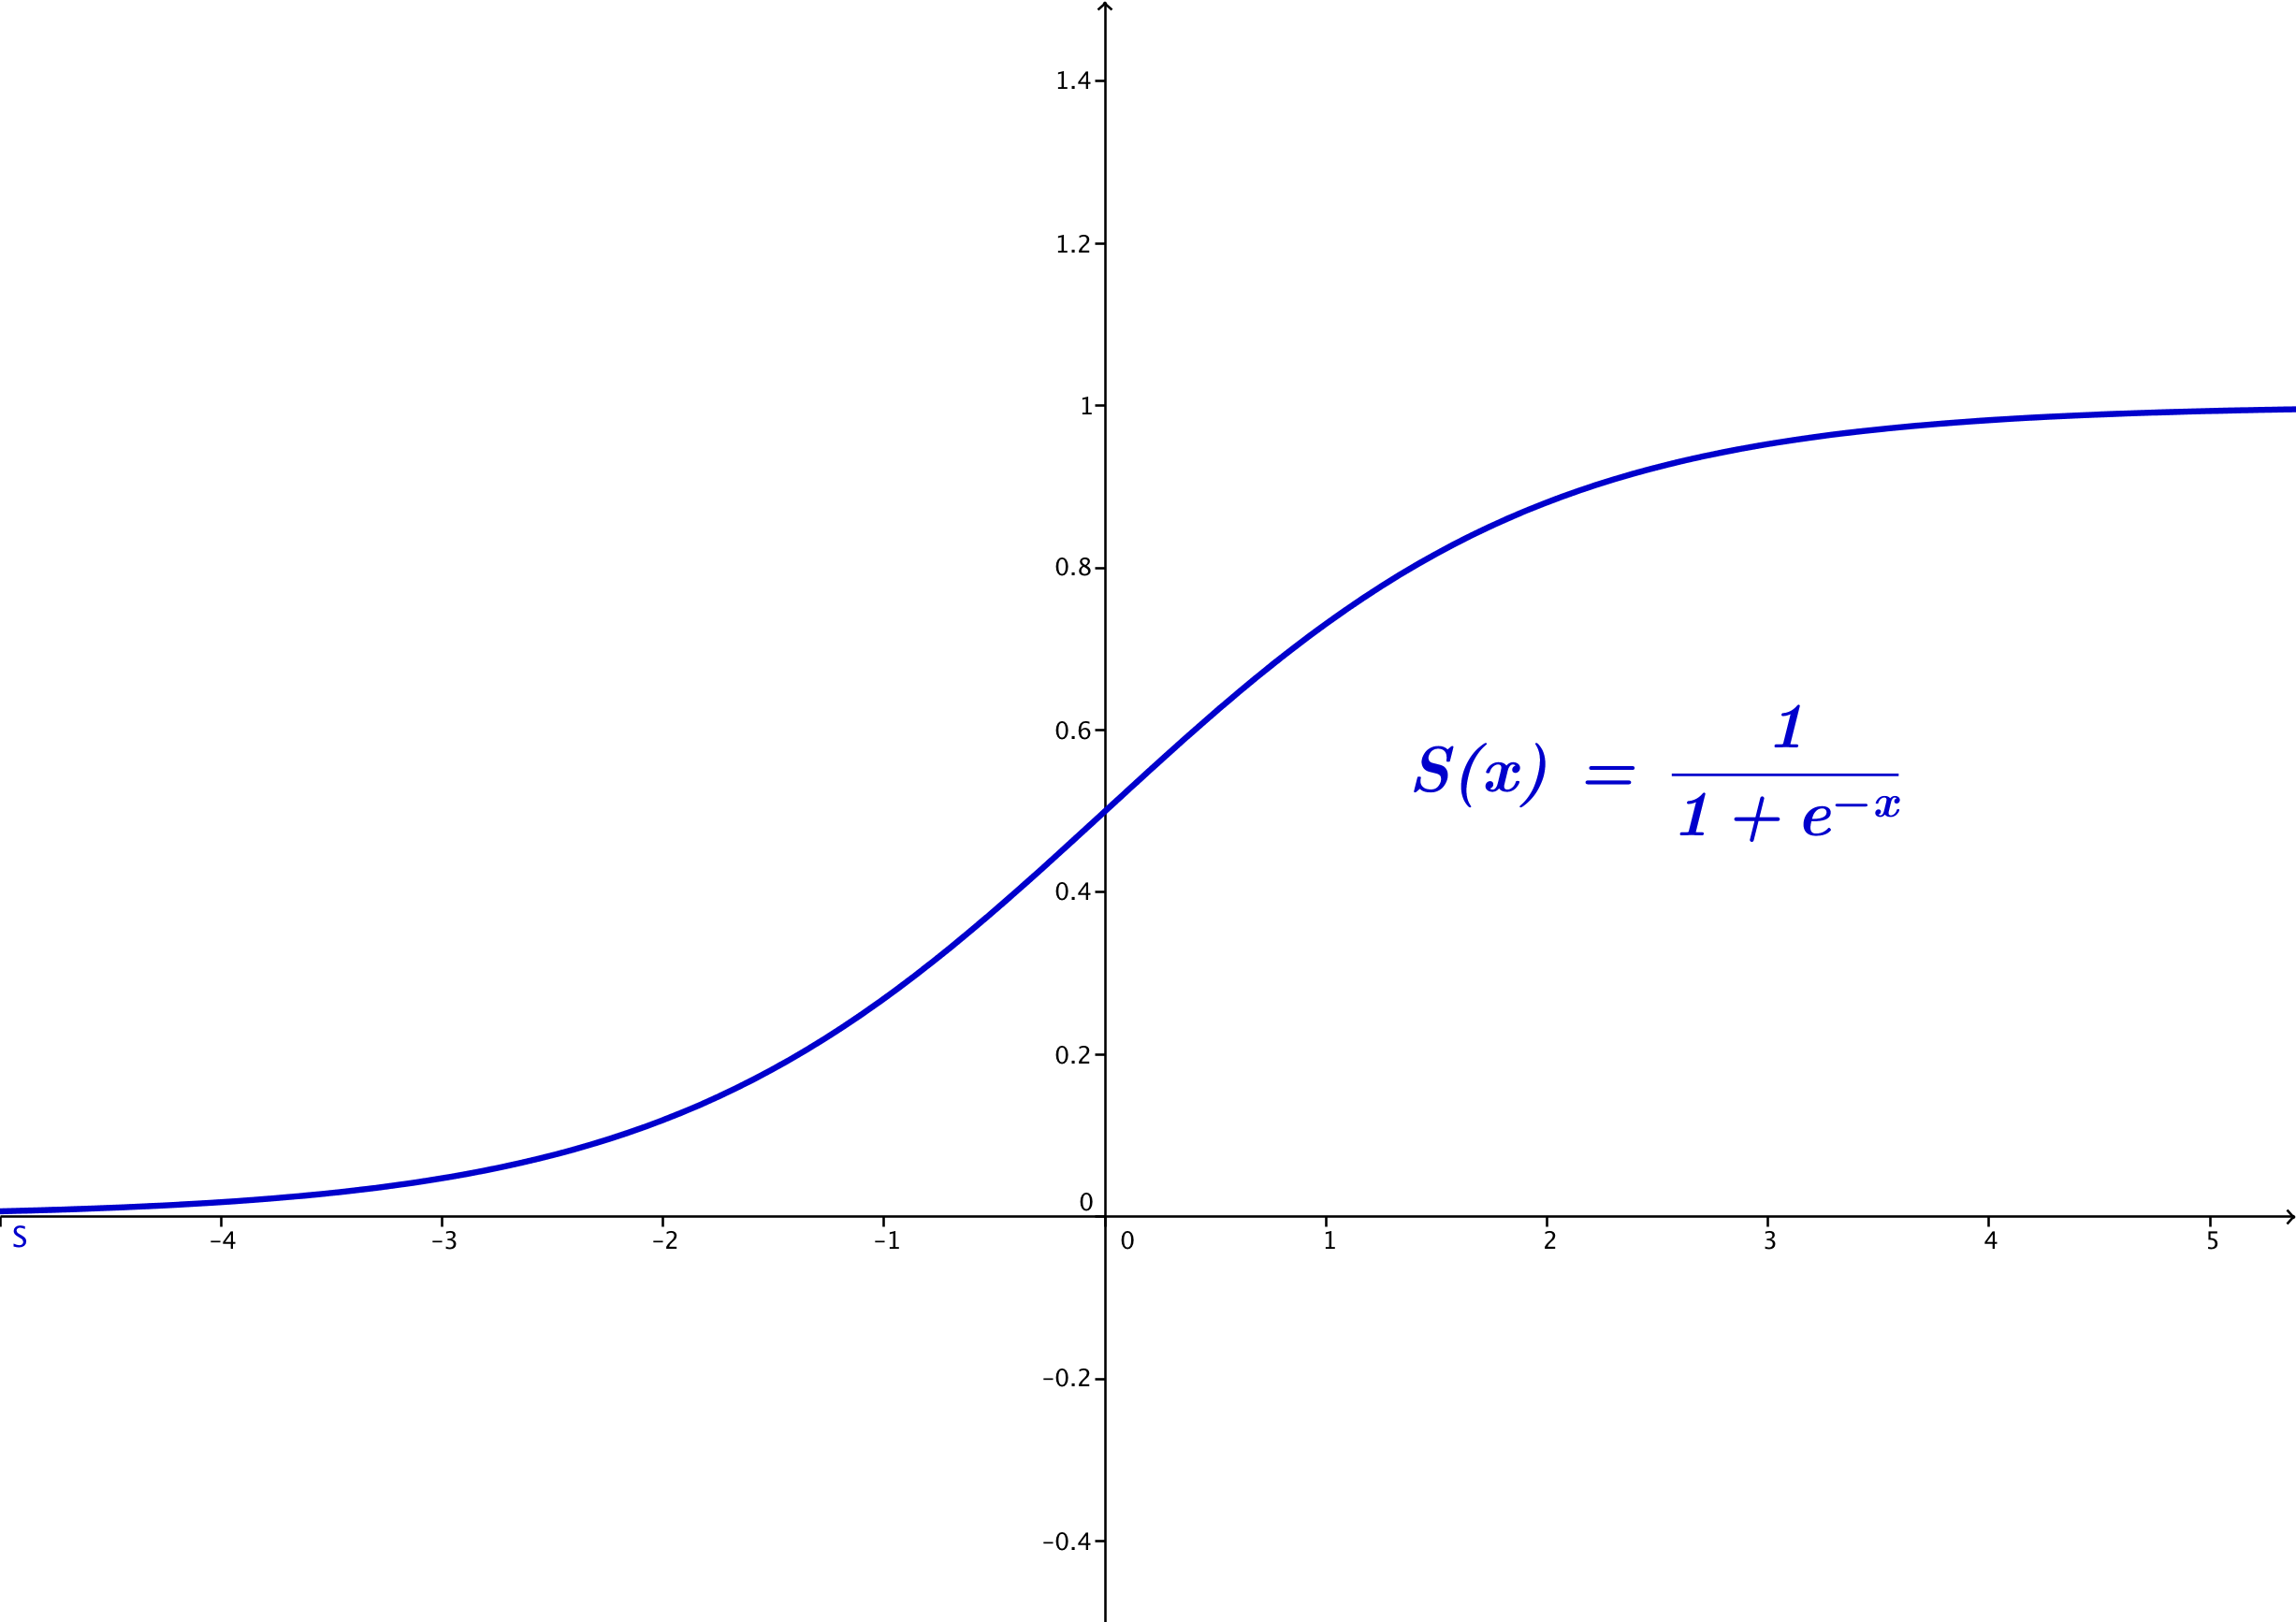
\includegraphics{Sigmoid}\centering
\end{figure}\\
Om vi nu istället föreställer oss ett neuron som endast tar emot en indata och som har en bias som är noll kommer summan av indata och bias vara $\sum_{i=1}^{n} {w_ix_i} -0=wx$ och aktiveringsfunktionen vara $\sigma(wx)$. Om vi nu ändrar på vikten påverkar det funktionens lutning när den går från $0$ till $1$ men förändrar inte dess läge i x-led som man kan se i det vänstra exemplet. Om vi nu håller vikten $w$ konstant och ändrar biasnodens värde är lutningen konstant men funktionen förflyttar sig i x-led som man kan se i det högra exemplet.
\begin{figure}[ht]
% 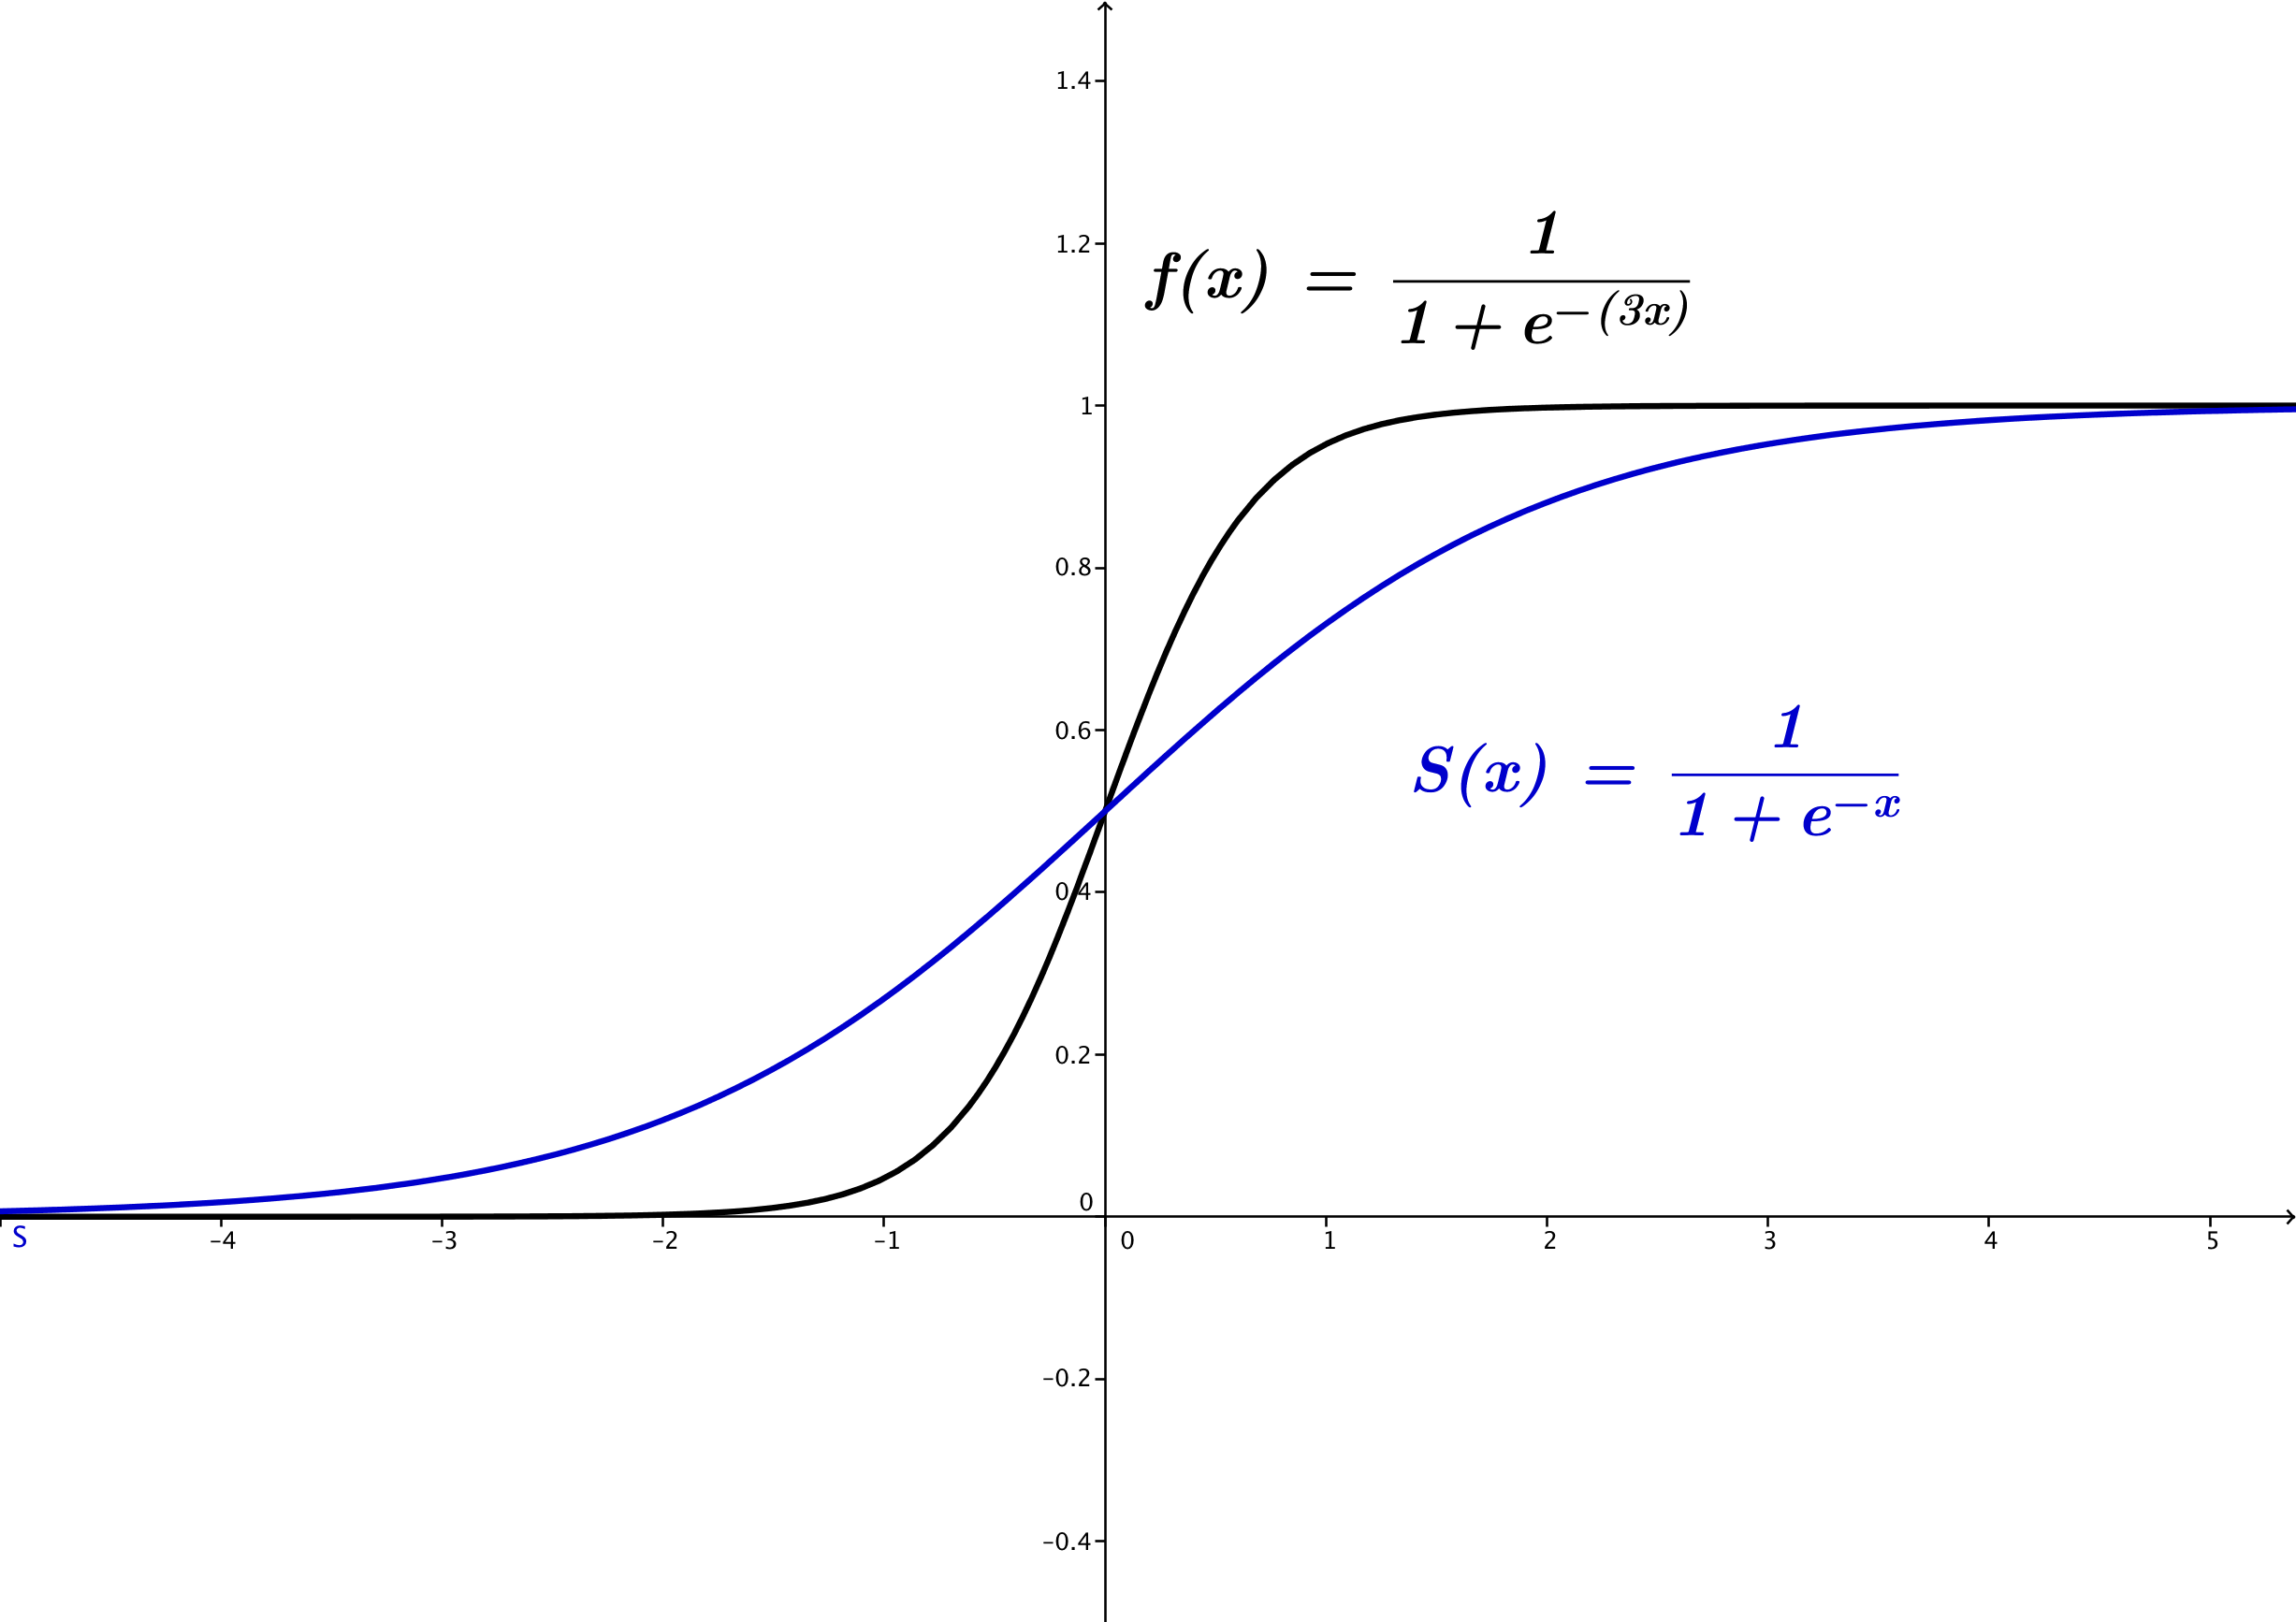
\includegraphics[width=0.5\textwidth]{Sigmoidw}
% \rule{.6pt}{5.7cm}%
% 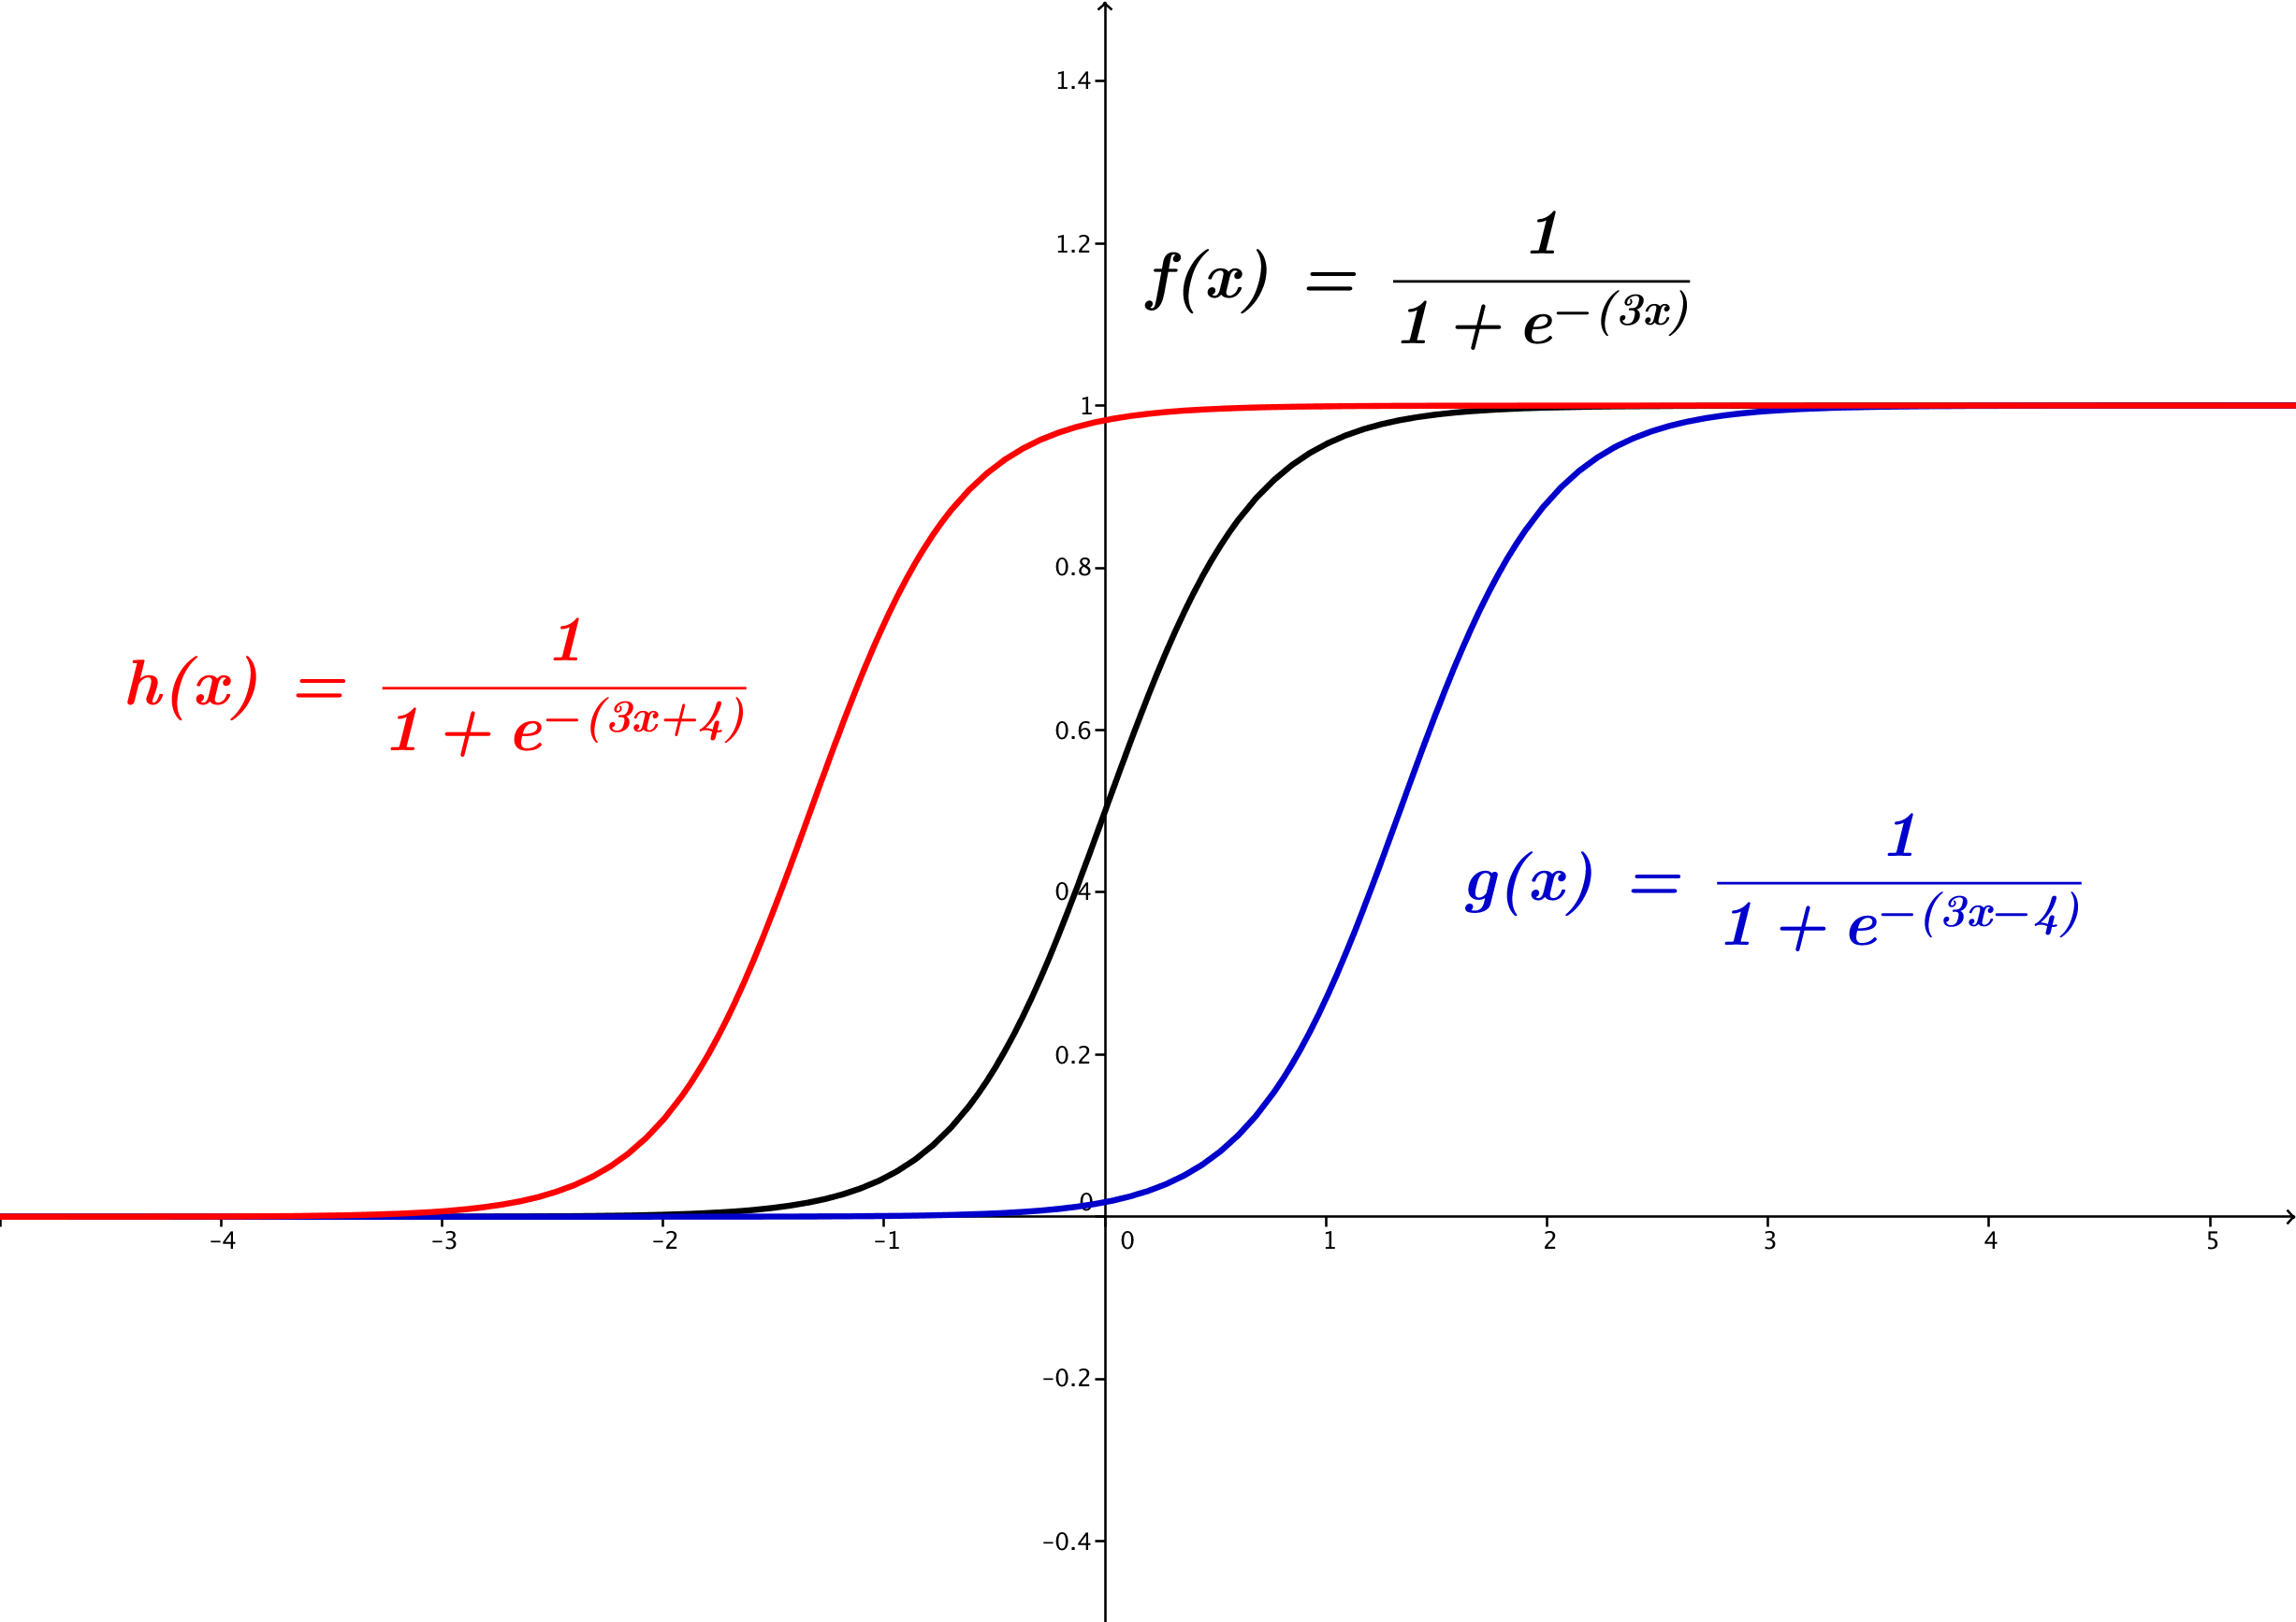
\includegraphics[width=0.5\textwidth]{Sigmoidb}
\fbox{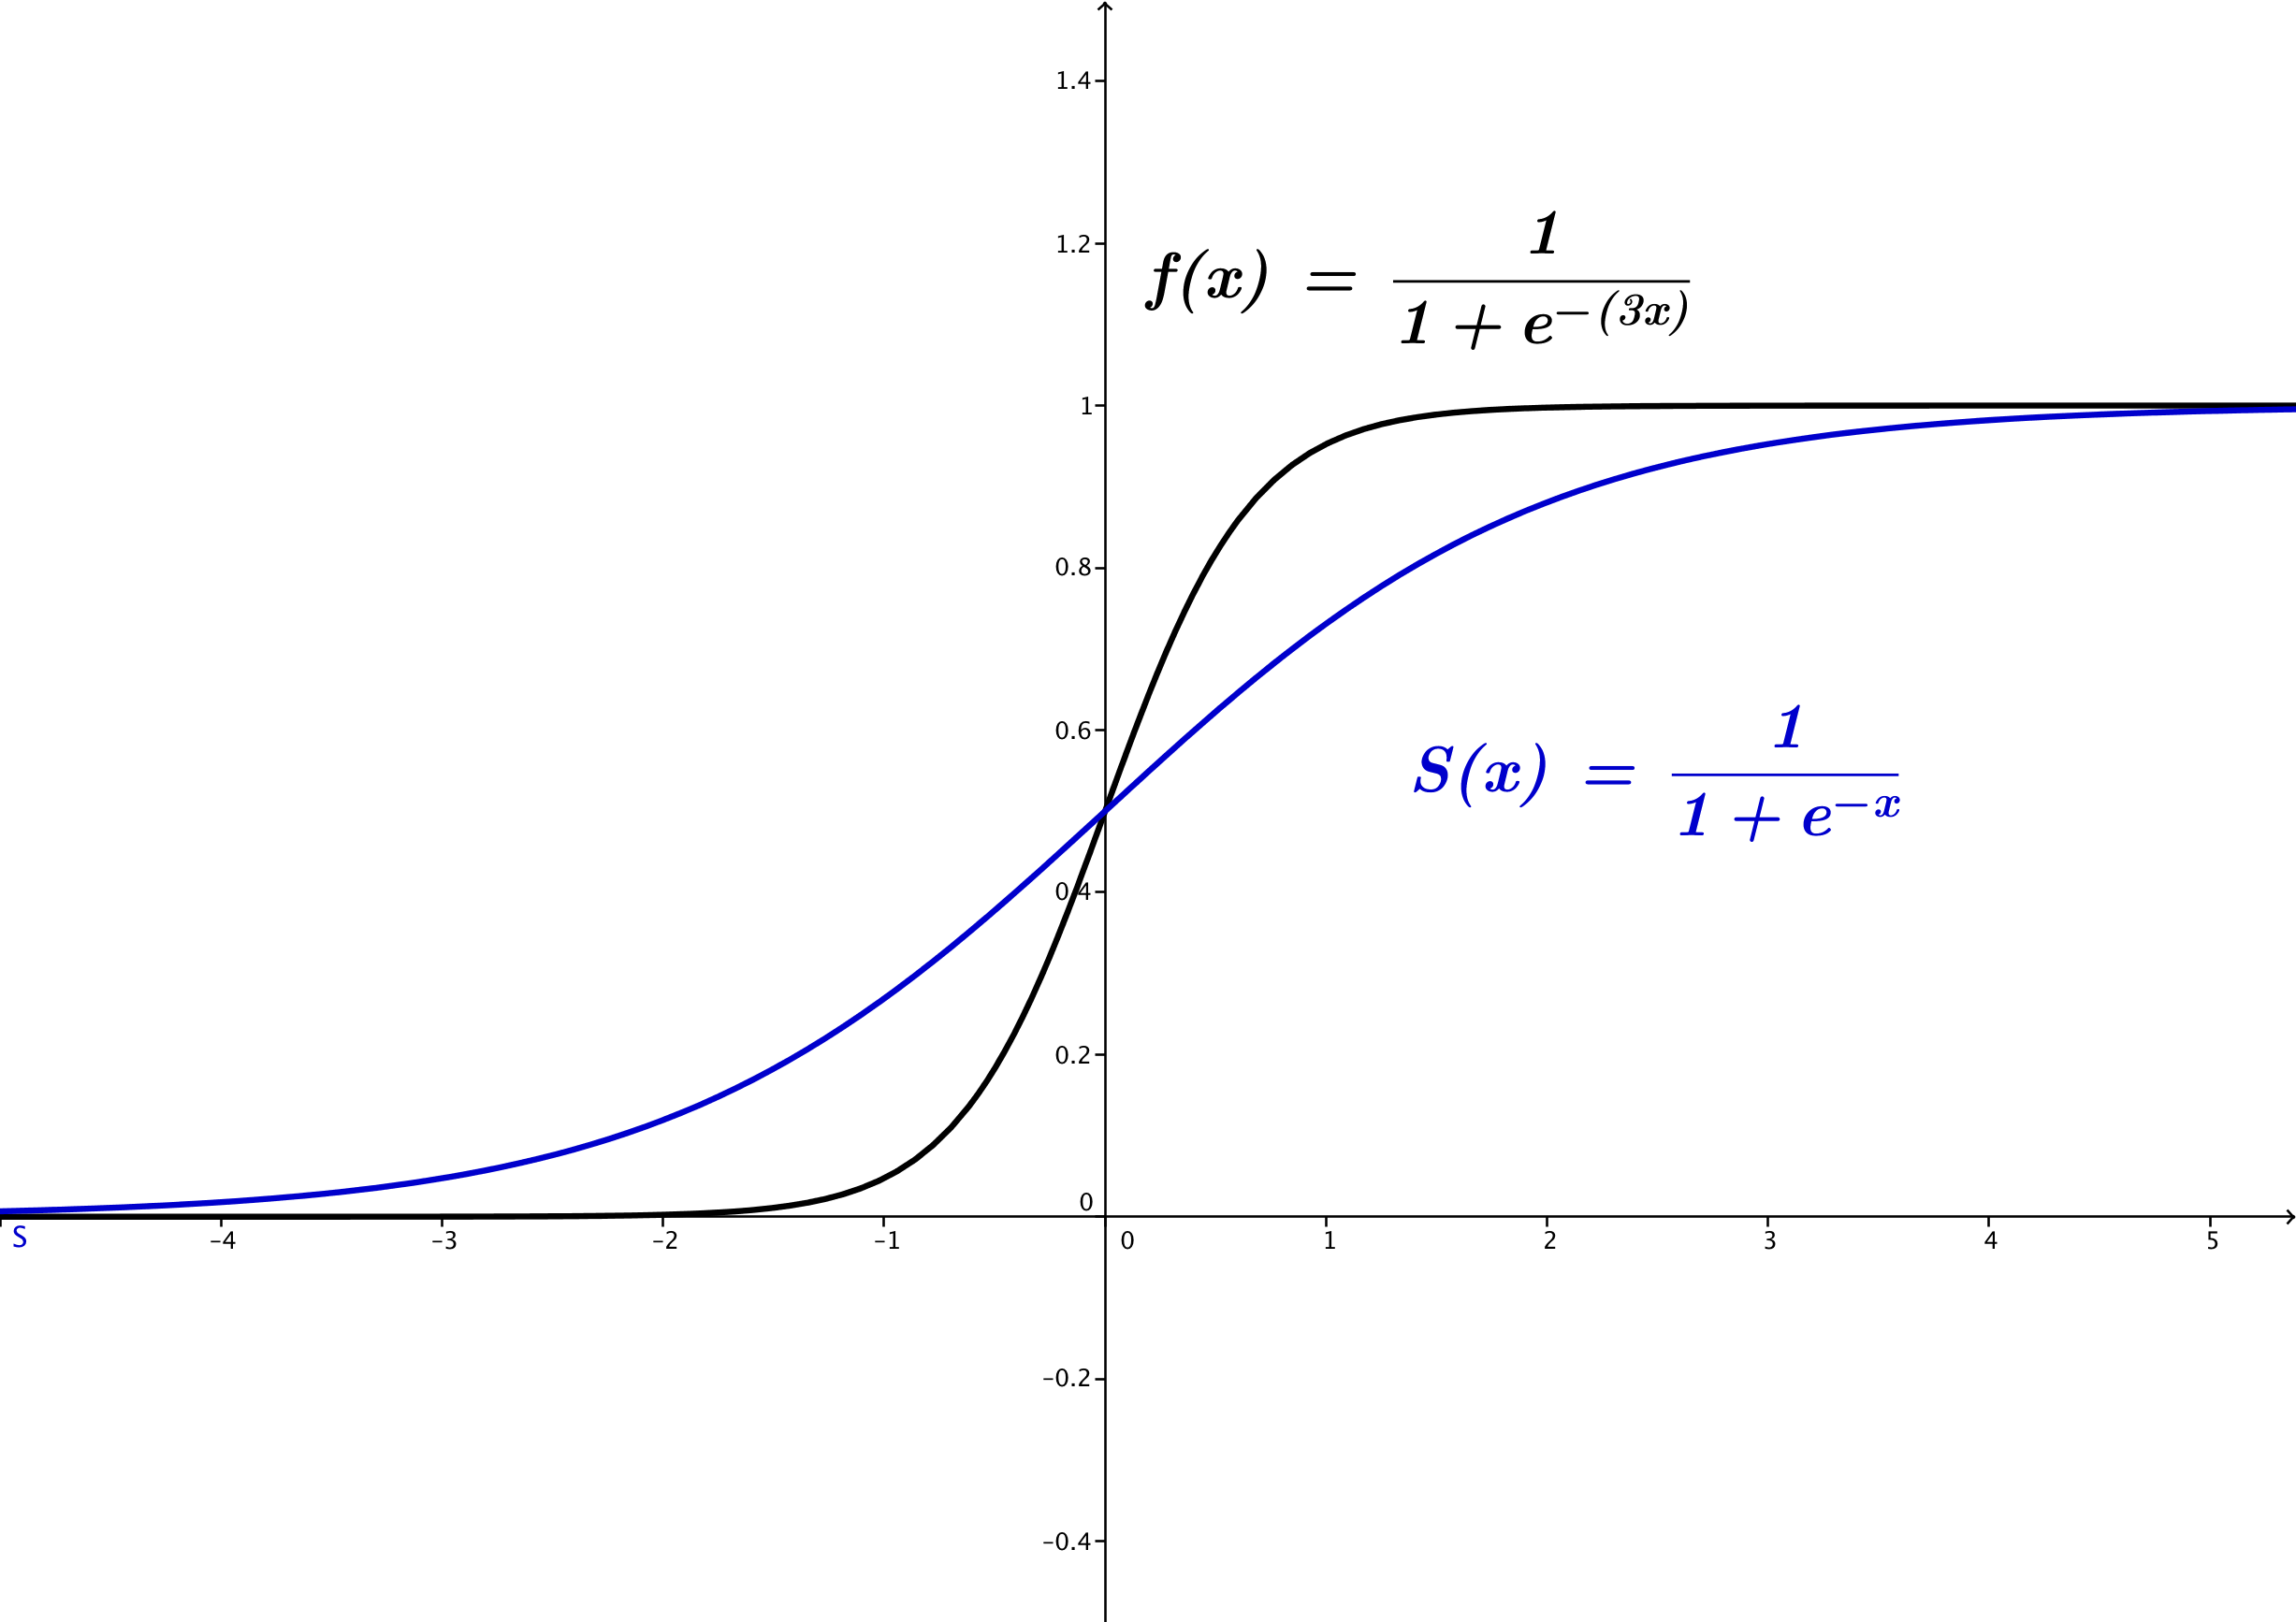
\includegraphics[width=0.5\textwidth]{Sigmoidw}}
\fbox{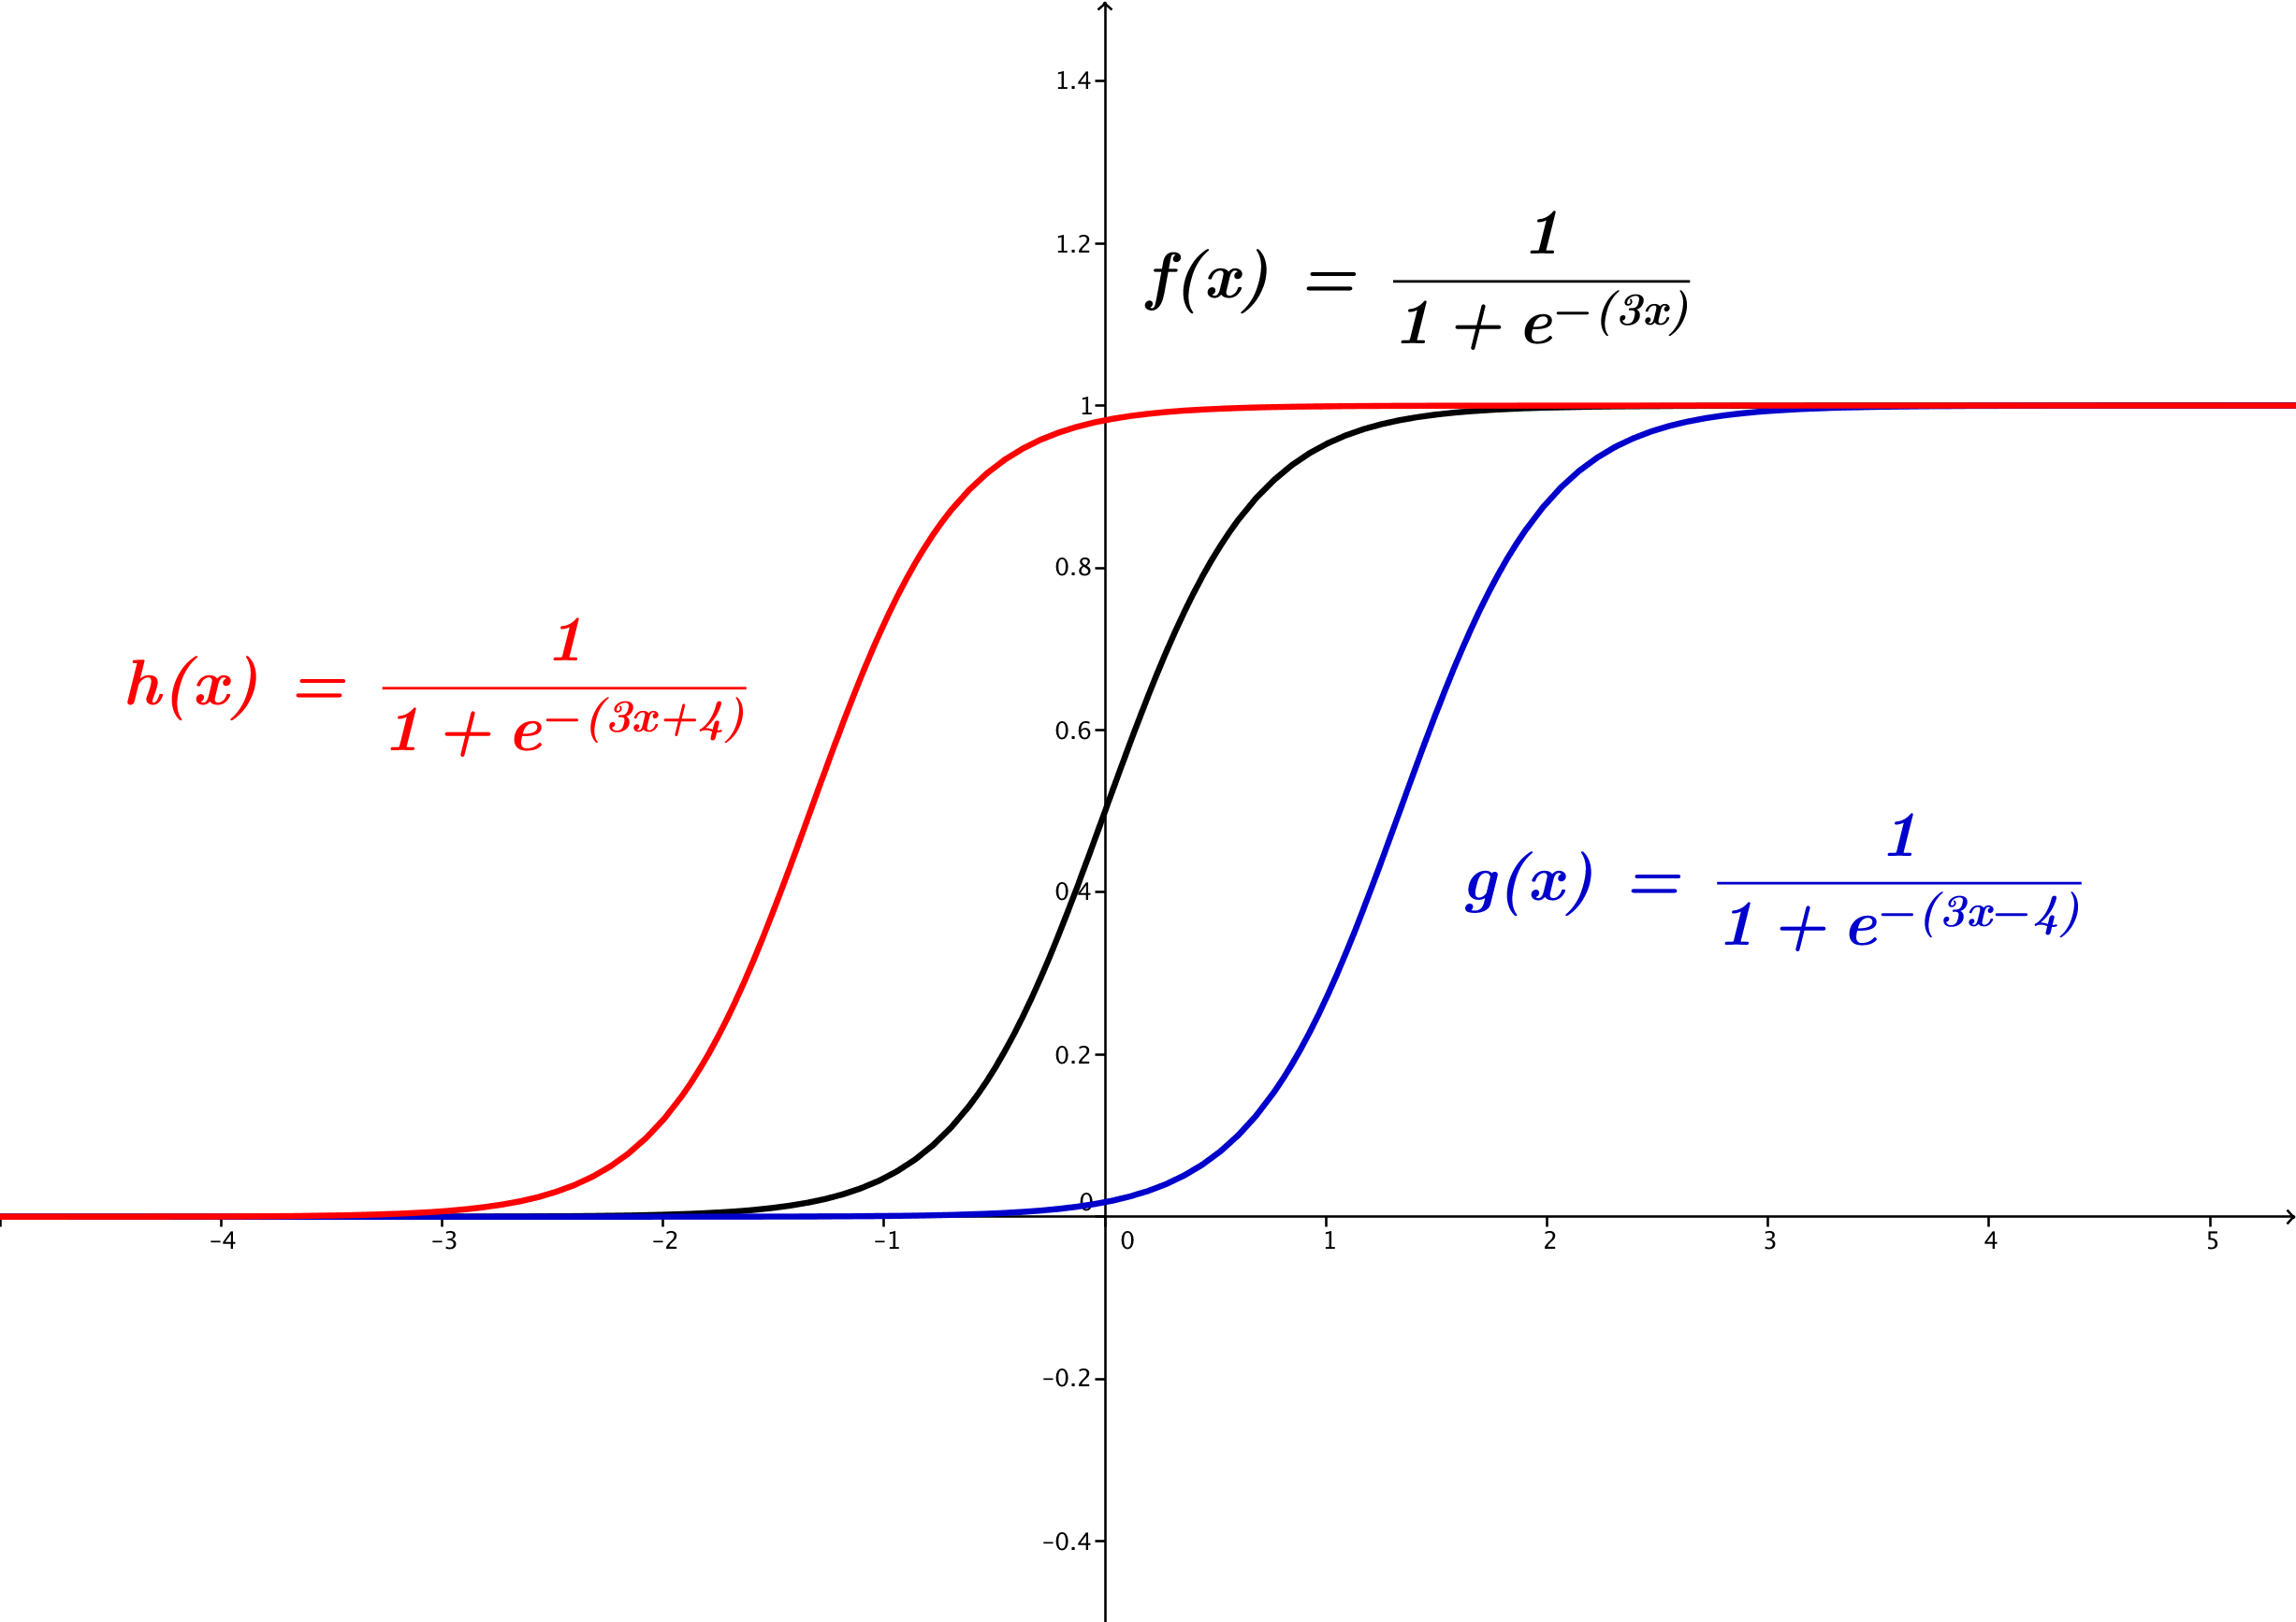
\includegraphics[width=0.5\textwidth]{Sigmoidb}}
\end{figure}


NN kan alltså använda biasnodens konstanta utdata för att justera sitt läge längs en axel. Biasnoder i samspel med flera lager innebär att man kan skapa mycket avancerade funktioner.

\subsubsection{Inlärningsalgoritmen}
Det finns olika sätt att angripa problemet med att få NN att lära sig och bli bättre. Det finns ett antal olika inlärningsalgoritmer men den vanligaste är backpropagation med hjälp av gradientsökning.

\paragraph{Backpropagation}\hspace{0pt}\\
Backpropagation (BP) är en förkortning av \emph{``Backward propagation of errors''} \autocite{BP} som uppkom under 1970 talet men betydelsen av algoritmen var inte helt förstådd tills 1986 när David Rumelhart och Ronald Williams skrev en artikel angående dess effektivitet för många NN \autocite{NNDL}. BP användersig av det som man kallar för övervakad inlärning vilket innebär att man tillhandhåller NN ett facit för sin träningsdata så den kan jämföra med det resultat som den själv fått. BP är en vanlig inlärningsmetod för NN och används tillsammans med en optimiserings metod som t.ex. gradient sökning. Gradient sökning är en optimiseringsalgoritm som söker att hitta en minpunkt för en funktion genom att gå ett antal steg som är negativt proportionerligt mot derivatan av en funktion\autocite{GD}. I fallet med BP resulterar det i att man söker att minimera errorfunktionen mellan NN:s resultat och facit för inlärningsdata.
BP algoritmen fungerar genom att man först ger NN indatan som den får bearbeta och producera ett resultat. Sedan beskriver man en errorfunktion baserad på det önskade resultatet och det faktiska resultatet t.ex. funktionen \\Mean Square Error ($MSE = \dfrac{(y-t)^2}{2}$). \\Därefter gås hela nätverket igenom baklänges och ändrar vikterna enligt principen för gradient descent genom att minska vikterna och biasnoderna med en inlärningsfaktor multiplicerat med derivatan för errorfunktionen vid den noden. Inlärningsfaktorn kan vi alltså använda för att beskriva hur stora ändringar vi ska göra varje gång vilket motsvarar hur snabbt nätverket lär sig. En mer fördjupad matematisk förklaring till hur och varför den funkar finns med som bilaga \ref{BPN}.

\subsubsection{Nätverkets storlek}
Storleken på nätverket kommer att vara beroende av flera olika faktorer den som väger tyngst är komplexiteten för BP och antalet lager.
\paragraph{Antal lager}\hspace{0pt}\\
Antalet lager som ska användas för ett nätverk är mycket svårt att bedömma då det beror på många faktorer som antalet indata, om funktionen är sammanhängande, vilken aktiveringsfunktion som används i neuronera os.v. När antalet lager i ett nätverk ökar kan nogrannheten öka men det finns ingen försäkring på att det kommer göra det. Det finns t.ex. två olika modeller för antalet lager. NN med få lager kallas för ytliga nätverk och de NN som har flera dolda lager mellan indatalagret och utdatalagret kallas för djupa nätverk\autocite{DL}. De ytliga nätverken är lättare att programmera och arbeta med eftersom att algoritmen för inlärning blir lättare tack vare att de består av ett fåtal dolda lager (1-2). De kan approximera de flesta funktioner\autocite{SLA} men nackdelen är att det kan vara svårare för ytliga nätverk att vara generaliserade eftersom att de kan kräva stora mängder träningsset och noder i de dolda lagren. För vissa funktioner fungerar de lika bra som de djupa nätverken som är svårare att implementera\autocite{SLA} vilket innebär att ytliga nätverk fortfarande är mycket användbara.  

\paragraph{Inlärning}\hspace{0pt}\\
Den algoritm för backpropagation som kommer att beskrivas är anpassad för ett nätverk med 3 lager (indatalager, dolt lager och utdatalager) eftersom att det räcker med ett dolt lager för de flesta NN.\autocite{StackExchange}\autocite{SLA}  Algoritmen är beskriven i pseudokod i bilaga \ref{Pseudo} och kommer att ha en tidskomplexitet på $\mathcal{O}(|I\cdot D+U\cdot D|) = \mathcal{O}(|W|)$ där $|W|$ betecknar storleken av mängden av alla vikter och $I,D,U$ är indata, dolda och utdatalagret för nätverket enligt bilaga \ref{BPC} som baseras på principen om gradient descent \autocite{GD}.

\paragraph{Antal noder}\hspace{0pt}\\
När det kommer till antalet noder i varje lager finns det några som har försökt skapa tumregler för hur många noder som ska användas \ref{FAQ}. Sanningen är att det är en otroligt komplicerad uppgift att komma fram till hur många noder som ska användas eftersom att det är nästintill individuellt för varje NN. Exempelvis har vi här ett nätverk som beräknar AND (vänster) och ett nätverk som beräknar XOR (höger). AND returnerar $1$ om man ger den $[1,1]$ som input och $0$ om man ger den $[1,0],[0,1],[0,0]$. XOR returnerar $1$ om den får $[1,0] eller [0,1]$ och $0$ annars. Båda dessa funktioner kan verka någorlunda simpla men skillnaden är att XOR inte går att träna om det inte har 2 noder i det dolda lagret medan AND kan tränas med endast $1$ nod i det dolda lagret. 
\begin{figure}[ht]
\centering
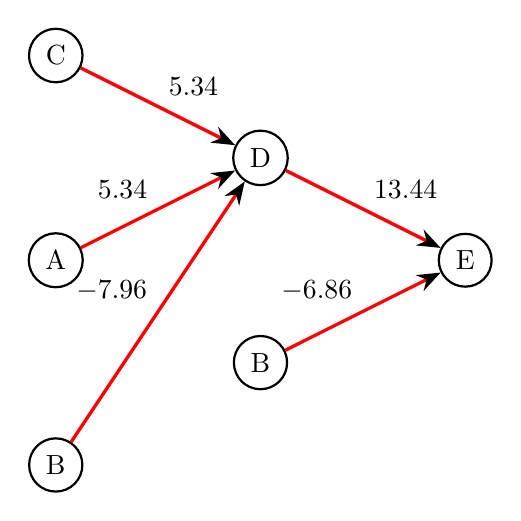
\begin{tikzpicture}[scale=1.3,auto]
\begin{scope}[every node/.style={circle,thick,draw}]
    \node (A) at (0,-2) {B};
    \node (B) at (0,0) {A};
    \node (C) at (0,2) {C};
    \node (D) at (2,-1) {B};
    \node (E) at (2,1) {D};
    \node (F) at (4,0) {E} ;
\end{scope}

\begin{scope}[>={Stealth[black]},
              % every node/.style={fill=white,circle,font=\small},
              % every node/.style={font=\small}
              every edge/.style={draw=red,very thick}]
    \path [->] (A) edge node {$-7.96$} (E);
    \path [->] (B) edge node {$5.34$} (E);
    \path [->] (C) edge node {$5.34$} (E);
    \path [->] (D) edge node {$-6.86$} (F);
    \path [->] (E) edge node {$13.44$} (F);
\end{scope}
\end{tikzpicture}
\hspace{1cm}
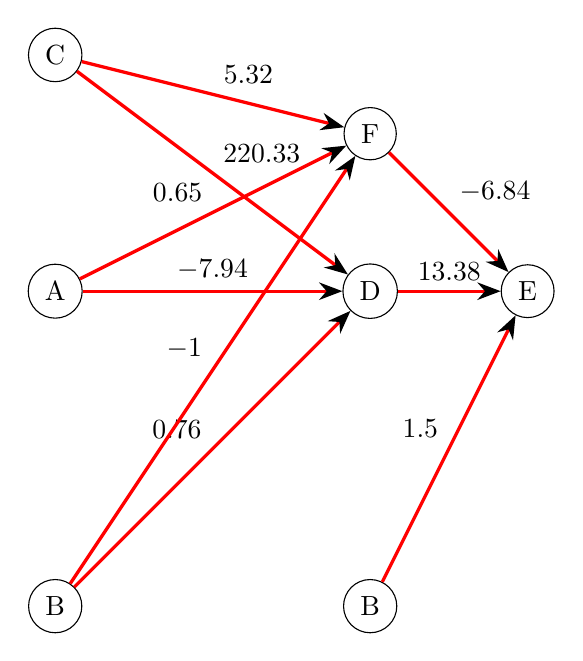
\begin{tikzpicture}[auto]
\begin{scope}[every node/.style={circle,draw}]
    \node (A) at (0,-4) {B};
    \node (B) at (0,0) {A};
    \node (C) at (0,3) {C};
    \node (D) at (4,-4) {B};
    \node (E) at (4,0) {D};
    \node (F) at (6,0) {E} ;
    \node (G) at (4,2) {F} ;
\end{scope}

\begin{scope}[>={Stealth[black]},
              every edge/.style={draw=red,very thick}]
    \path [->] (C) edge node {$220.33$} (E);
    \path [->] (C) edge node {$5.32$} (G);
    \path [->] (B) edge node {$-7.94$} (E);
    \path [->] (B) edge node {$0.65$} (G);
    \path [->] (A) edge node {$0.76$} (E);
    \path [->] (A) edge node {$-1$} (G);
    \path [->] (E) edge node {$13.38$} (F);
    \path [->] (G) edge node {$-6.84$} (F);
    \path [->] (D) edge node {$1.5$} (F);
\end{scope}
\end{tikzpicture}
\end{figure}
Eftersom att det är så svårt att välja antalet noder kan man dock använda sig av vissa tumregler för att påbörja testerna och sedan optimera vid behov. T.ex. kan man använda en tumregel som säger att antalet noder i det dolda lagret ska vara medelvärdet på indatalagret och utdatalagret \autocite{StackExchange} och anpassa därefter när det behövs \ref{FAQ}

\subsubsection{Data}
För att vi ska kunna träna nätverket måste vi ge den indata och korrekt utdata som kan användas i errorfunktionen. Vi generar en mängd med testdata av\emph{``rena toner''} som genereras enligt $y=\sin(f_{not}*2\pi t)$.\autocite{Wave}\\
$f_{not}$ är frekvensen för respektive not av de 87 tonerna A0 t.om. B7 och $t$ är tiden i sekunder. C8 som är den högsta frekvensen svänger såpass fort så att det blir svårt att skapa bra genererad data. Dessutom dör tonen ut fort på pianot vilket gör att det finns stora risker att det blir oanvändbar mätdata.

% Kristoffer
Ljud är tryckvågor. Dessa går naturligtvis inte att spara i rå form på en dator. Detta då en dator enbart kan spara binära värden och inte fysiska vågor. Därför måste man för att kunna arbeta med ljudvågor på en dator representera de i binär form. Det finns en hel del sätt att göra detta. Den vanligaste metoden är att spara det som en mängd data punkter som beskriver kompressionen hos ljudvågen. 
För att spela in ljud måste man interagera med en mikrofon. Vi bestämde oss för att använda SFML. SFML är ett gränssnitt mellan program och datorns auditiva samt grafiska hårdvara.  
I projektet är vi främst intresserade av ljudens frekvens eftersom man inom musiken kategoriserar ljud som toner efter deras frekvens. Ett fenomen som uppkommer när man spelar olika instrument är att man får svävningar vilket gör att inspelade toner får en annorlunda form gentemot rena toner. Svävningar är när två toner med likartad frekvens spelas samtidigt så uppfattas de av örat som en och samma mellanliggande ton\autocite{BEAT}. Detta kan förklaras enkelt med hjälp av matematik: Sin(a + b) + Sin(a - b) = 2 * Sin(a) * Cos(b). Då ser vi även att vågen kommer gå upp och ner i amplitud över ett större intervall, ty allt multipliceras med Cos(b). 

Eftersom att pianot som ett musikinstrument är byggt så att det låter annorlunda jämfört med en t.ex. stämgaffel vars ljudvåg är mer snarlik en perfekt sinusvåg innebär det att vår genererade data kommer att skilja sig ifrån den inspelade. Detta kan bättre illustreras med de två graferna nedan som föreställer den genererade tonen och den inspelade tonen av A4 440Hz. 
\begin{figure}[ht]
\fbox{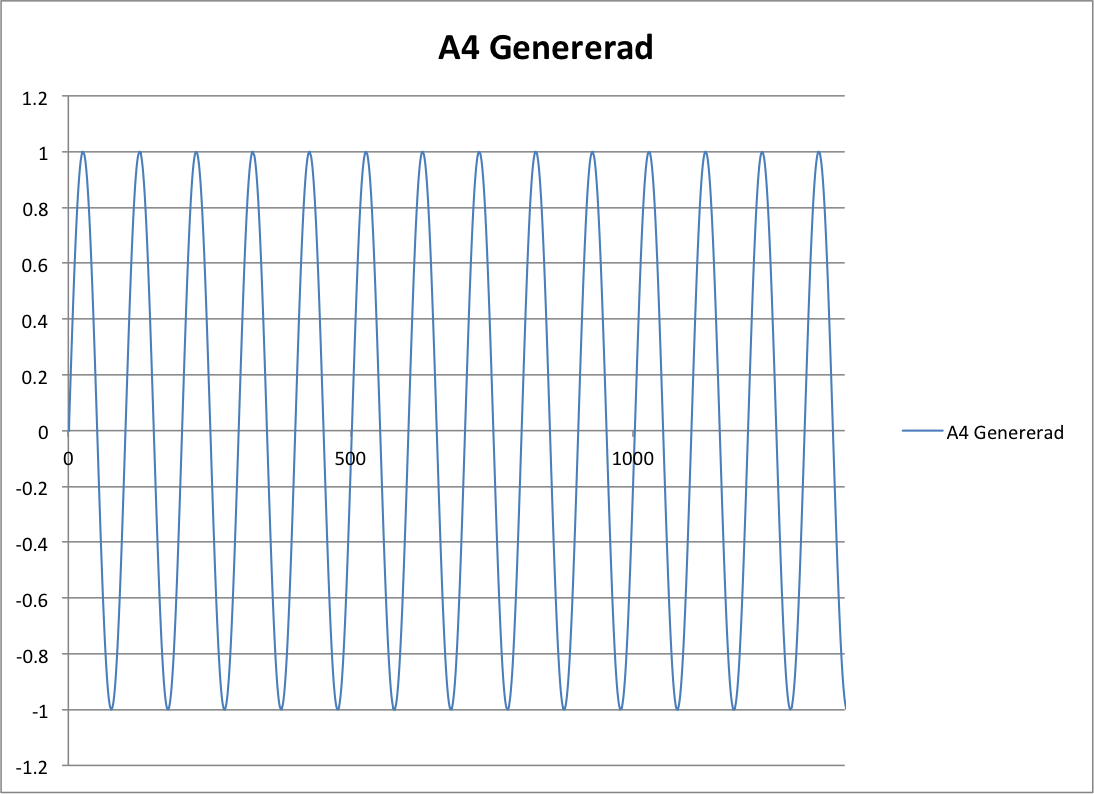
\includegraphics[width=0.5\textwidth]{A4gen}}
\fbox{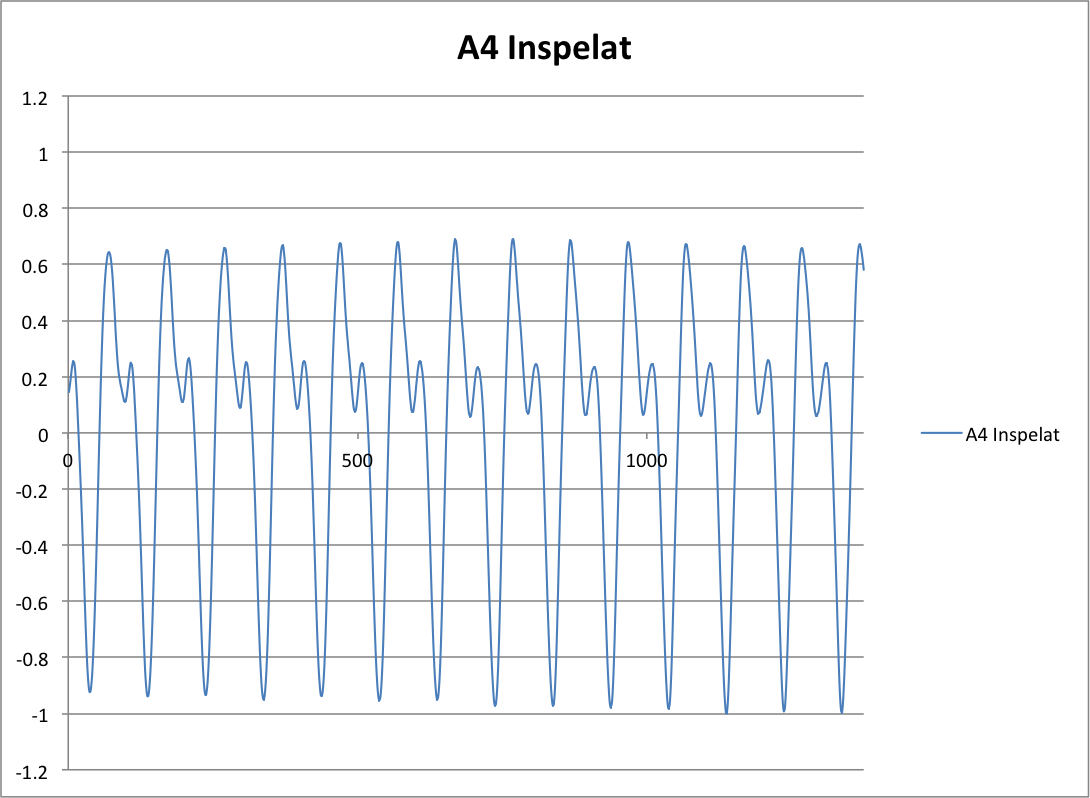
\includegraphics[width=0.5\textwidth]{A4p}}
\end{figure}

Inlärningsdata är inspelad i ett tyst rum med minimalt med bakgrundsbrus på ett piano. 
Det finns ett antal sätt att representera ljud på en dator. Den vanligaste formen är att spara det som en mängd datapunkter som beskriver amplituden på ljudvågen.
För att spela in ljud måste man interagera med en mikrofon. Vi bestämmde oss för att använda SFML. SFML är ett gränssnitt mellan program och datorns auditiva samt grafiska hårdvara. 

Vi ville minimera antalet faktorer nätverket måste handskas med. Vi normaliserade ljudvågens amplitud så att alla toppar och dalar alltid låg mellan -1 och 1. Datan som spelas in delas upp i mindre segment, i varje av dessa segment väljs värde som ligger längst ifrån x-axeln och dividerar alla andra värden med dess absolutbelopp och detta ger en kurva som förhoppningsvis ger högre vikt på frekvensen än det annars skulle gjort. Detta eftersom att när man spelar in tonerna är det svårt att spela in alla med en konstant ljudstyrka. t.ex. avtar ljudstyrkan allt eftersom att tiden går. Eftersom att NN tar emot flyttal eller decimaltal innebär det att det skulle kunna resultera i att NN returnerar olika toner om man spelar samma ton med olika ljudstyrka eftersom att högre ljudstyrka ger högre amplitud vilket ger ett högre indatatal åt det NN.
% Slut





% Diskussion
% Så det finns ett fåtal problem som kan uppkomma i vårat projekt på grund av ljud.
% Först så har vi problemet med normalsering. Vi har bestämmt att normalisera våran inspelade data för att få alla värden att ligga mellan -1 och 1. Detta beslut togs då vi ville eliminera en faktor av arbete för nätverket så att den bara behöver tänka på frekvensen. Osäkerheten låg i hur vi skulle normalisera. Till en början ville vi normalisera över hela den inspelade datan. Att normalisera med denna metod är dock helt onödigt då vi senare delar upp filen i en massa små filer. Ljudet går gradvis ner i styrka över tid vilket innebär att de senare delarna inte kommer vara normaliserade och vi är tillbaka på ruta noll. Men om vi däremot bestämmer oss för att normalisera över intervallen vi sedan skär ut så kommer vi få åtminstone få att alla segment vi jobbar med är normaliserade. Problemet vi fann med denna metod är att den högsta punkten i intervallet inte nödvändigtvis är en top på en våg. Detta kan möjligtvis komma att försvåra saker för nätverket.
% Ett annat problem vi kom att tänka på är att var att de inspelade tonerna kommer innefatta svävning medan de genererade inte innefattar det. Vi är osäkra hurvida nätverket kan klara av det problemet.




% \setcounter{secnumdepth}{1}

\subsection{Syfte och frågeställningar}

Syftet med vår undersökning är att lära oss mer om hur NN fungerar och hur man kan anpassa dem för olika uppgifter. Vi vill också undersöka hur effektivt nätverket är eftersom att en av de stora begränsningarna med NN var att de krävde mycket processorkraft vilket gjorde att forskningen stannade upp ett tag runt 1970-talet tills det att man kunde tillverka datorer som kunde utföra fler processer per sekund än tidigare. Vi är också intresserade av hur bra vårt nätverk blir på att gissa rätt (samt hur liten vi kan få errorfunktionen att bli för alla noder), hur lång tid det tar för det att lära sig och vad det har för begränsningar.

\break
\subsection{Frågeställningar}
\begin{enumerate}
\item Hur kan man anpassa ett neuralt nätverk för att känna igen toner?
\item Hur träffsäkert blir nätverket?
\item Vad är det för tidskomplexitet på nätverket? (körning, inlärning)
\end{enumerate}

\subsection{Avgränsningar}
Från början var arbetet tänkt att omfatta röstigenkänning men vi gjorde därefter om det till ljudigenkänning. Då det kändes för brett och ospecificerat gjorde vi det till ton-igenkänning. Inom ton-igenkänning vill vi inkludera tonerna för främst piano och hur nätverkets påverkas av att pianots ljudvåg har andra vågor som är superpositionerade på tonen. \\
På grund av tidsbrist har vi behövt strukturera om och testa ett nätverk som bara undersöker om den kan lära sig att se skillnad på A4 och C4 när det består av 3 lager och 4 lager och ett nätverk som undersöker om den kan särskilja 12 toner (C4-B4).

\section{METOD}

\subsection{Förklaring av Nätverket}
Nätverket består av en lagerstruktur. Lagren samlas i något som kallas ett lagerkluster, lagren innehåller noder. I varje lager finns det en så kallad bias-nod som alltid ger utdata 1. Varje nod (förutom bias-noden) innehåller en kant till alla noder i det tidigare lagret (inklusive bias-noden). Det första lagret representeras endast av en lista av utdata som går med viktning till det första dolda lagret.

% \subsubsection{Beräkning}
% En nod tar in indata från alla noder i det tidigare lagret. Den har en specifik viktning för varje nod i det tidigare lagret. Indata betäcknar vi som D och vikten som W. Vi använder sigmoidfunktionen: $$\phi = \frac{1}{e^{-{\sum_i{(W_i * D_i)}}}}$$ detta görs för alla noder i ett lager i taget sen sätts alla indata i nästa lager till utdatan till det tidigare lagret dvs $\phi$ för alla noder.

% \subsubsection{Träning}
% Nätverkets vikter initialiseras till mellan -0.5 och 0.5. Sedan tränas nätverket upp genom bakåtutbredning. Man använder flera data som tränar nätverket genom att köra det på de olika testdata som man har. Vi har generer 87 olika toner med förskutning i 31 olika steg som vi slumpmässigt väljer när nätverket tränas.

\subsubsection{Kodstruktur}
Koden består av ett klusterobjekt som innehåller en indatalista (som beskrivet tidigare) och en lista av lager. Varje lager innehåller ett antal noder som innehåller (som beskrivet tidigare) alla vikter till det tidigare lagret.

\subsection{Nätverken}
Eftersom att sigmoidneuronerna är enkla och mycket bättre än perceptronerna har de valts för att agera som aktiveringsfunktion för noderna och bygga upp nätverket för det. Målet för utdatanod $n\in\{1,2,3...86,87\}$ är att returnera $1$ om det är den tonen som spelas och annars returnera $0$.
% Tonerna är sparade i bokstavsordning vilket innebär att ton $1$ och $2$ inte motsvarar A0 och A\#0 utan A\#0 och A\#1.\\
Enligt teorin kommer antalet beräkningar förhålla sig mot antalet vikter och antalet noder i de olika lagren. Ljudet har spelats in med en hastighet på 44000 $Hz$ och eftersom att varje indatanod motsvarar en datapunkt kan nätverket inte använda ljudet som spelas in under en sekund då antalet beräkningar kommer öka väldigt snabbt nätverket består av 44000 noder i ett lager. Istället delas de inspelade datapunkterna upp i $32$ mindre segment vilket blir: \[\dfrac{44000}{32}=1375\] Alltså kommer nätverkets indatalager bestå av 1375 noder vilket är hanterbart utan att nätverket tillhandages för lite indata. \\
BP valdes som inlärningsalgoritm för alla nätverk eftersom att den är relativt enkel och fungerade tillräckligt bra för upplärning av AND och XOR nätverken. Inlärningen kan bromsas om vi hamnar i ett lokalt minimum\autocite{NNDL} men det är en risk som är svår att undvika oberoende av val av inlärningsalgoritm.
Den algoritm som kommer användas för BP är beskriven i pseudokod i bilaga \ref{Pseudo}. tonera dock att den bara är beskriven för nätverken med 3 lager. Vi bygger upp nätverket och sparar det så att det går att återskapa ifrån det vi hade tidigare. 


\subsubsection{Nätverk 1}
Nätverket bestod av 87 utdatanoder vilka representerade de 88 tonerna av pianot om man utelämnar C8. 
Det dolda lagret i det första nätverket har ungefär medelvärdet av utdata och indatalagrens noder (avrundat uppåt) alltså: \[\dfrac{1375+87}{2}=731\] Men för att ligga över medel använde vi $732$ noder. Nätverket tränades med en slumpad lista av genererade toner, ListN, som innehåller $10^5$ fall av 30 sekvenser för de 87 olika tonerna som har delats upp i $31$ mindre segment. Nätverket tränades med en inlärningsfaktor på 10,1,0.5,0.1. 
\subsubsection{Nätverk 2}
Efter det att Nätverk 1 misslyckades med att returnera korrekta svar ökas antalet nätverk i ett försök att anpassa nätverket. Det dolda lagret i det andra nätverket bestod av 7000 noder för att undersöka om det gav bättre resultat. 
\subsubsection{Nätverk 3}
Då Nätverk 2 inte heller lyckas testas ett nätverk som endast försökte skilja på A4 och C4. 
\subsubsection{Nätverk 4}
Efter det att även Nätverk 3 misslyckats testades ett 4-lagers nätverk som försökte skilja på A4 och C4. Nätverket bestod alltså av $1375$ indatanoder, $732$ dolda noder i det första dolda lagret, $732$ dolda noder i andra dolda lagret och 2 noder i utdatalagret. Nätverket tränades med den genererade listan \emph{BList.txt} som bestod $10^5$ testfall av de 30 sekvenser (av 31)genererade toner för A4 och C4 med en inlärningsfaktor $\alpha=0.2$. Nätverket testades sedan med en lista \emph{2outTL.txt} som gick igenom alla de 32 fallen av de inspelade tonerna för A4 och C4 respektive.
\subsubsection{Nätverk 5}
När Nätverk 3 lyckades skilja på A4 och C4 testades det att öka antalet utdatanoder till 12, alltså försökte det skapas ett nätverk som kunde skilja på tonerna i spannet C4-B4. Antalet dolda noder ökades också i varje lager eftersom att det är mer komplext att försöka känna igen 12 toner. Nätverket tränades med en slumpad lista \emph{12List.txt} med $10^5$ fall av de genererade tonernas 30 sekvenser (av 31). I första varvet av träning användes en inlärningsfaktor $\alpha=0.2$. Nätverket testades sedan med en lista \emph{TESTLIST.txt} som gick igenom alla de 32 fallen av de inspelade tonerna för C4 till B4 (resultat redovisas i bokstavsordning) respektive. \\I nästa varv användes \emph{12List.txt} igen men med en inlärningsfaktor $\alpha=0.1$. Sedan testades \emph{TESTLIST.txt}


% Ett basnätverk genereras så att det existerar en gemensam grund att träna nätverket från.






% \subsection{Tester}
% Fyra olika modeller för att lära upp det neurala nätverket kommer att testas. 
% \begin{itemize}[label={-}]
% \item Endast genererade toner (100-0)
% \item Först endast genererade toner, sedan endast inspelade toner (50-50)
% \item En jämn blandning av genererade och inspelade toner (100-0,0-100)
% \item Endast inspelade toner (0-100)
% \end{itemize}
% \subsubsection{100-0}
% När nätverket tränas med endast genererade data tränas det utifrån en redan slumpad lista, ListN, som innehåller $10^5$ sekvenser av de 87 olika tonerna som har delats upp i de 31 mindre segmenten.
% \subsubsection{100-0,0-100}
% För träningen med genererade och inspelade toner separat använder nätverket först ListN och sedan tränas det med en lista med endast inspelade toner (ListY) samma storlek som ListN.
% \subsubsection{50-50}
% För träningen med blandning av både inspelade och genererade toner skapas en lista som innnehåller lika många inspelade som generarade toner av samma storlek som ListN och ListY som kallas för ListM.
% \subsubsection{0-100}
% När nätverket endast ska tränas med inspelade data används listan ListY.
 

\newpage
\section{RESULTAT}
\begin{figure}[h!]
X-axel är tusental träningsfall\\
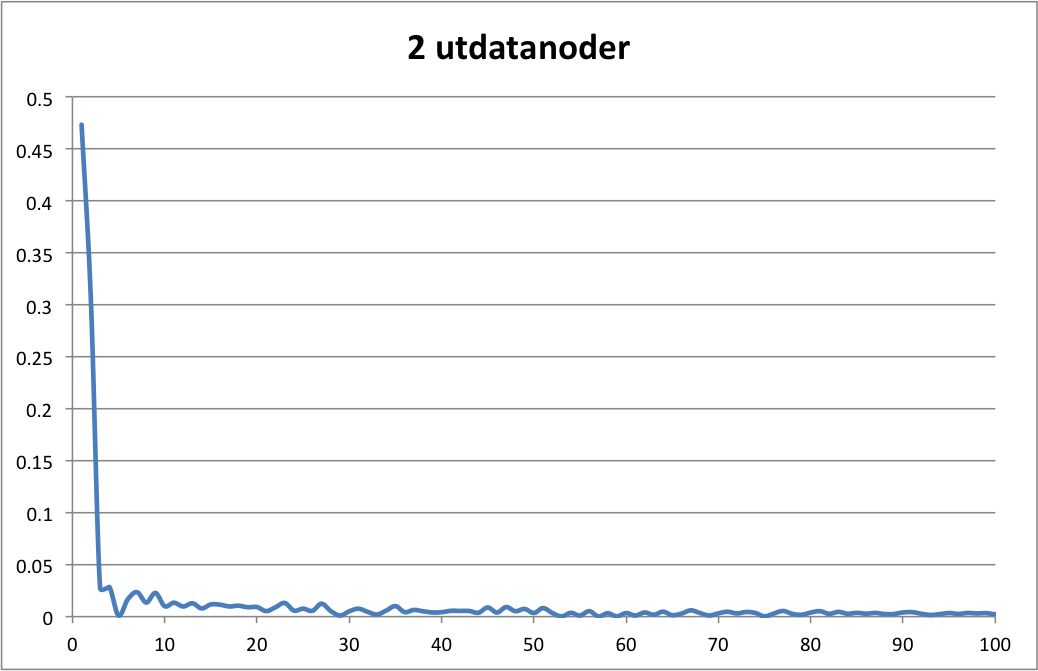
\includegraphics[width=\textwidth]{2outTR}
Visar utdata från förväntad nod för \\
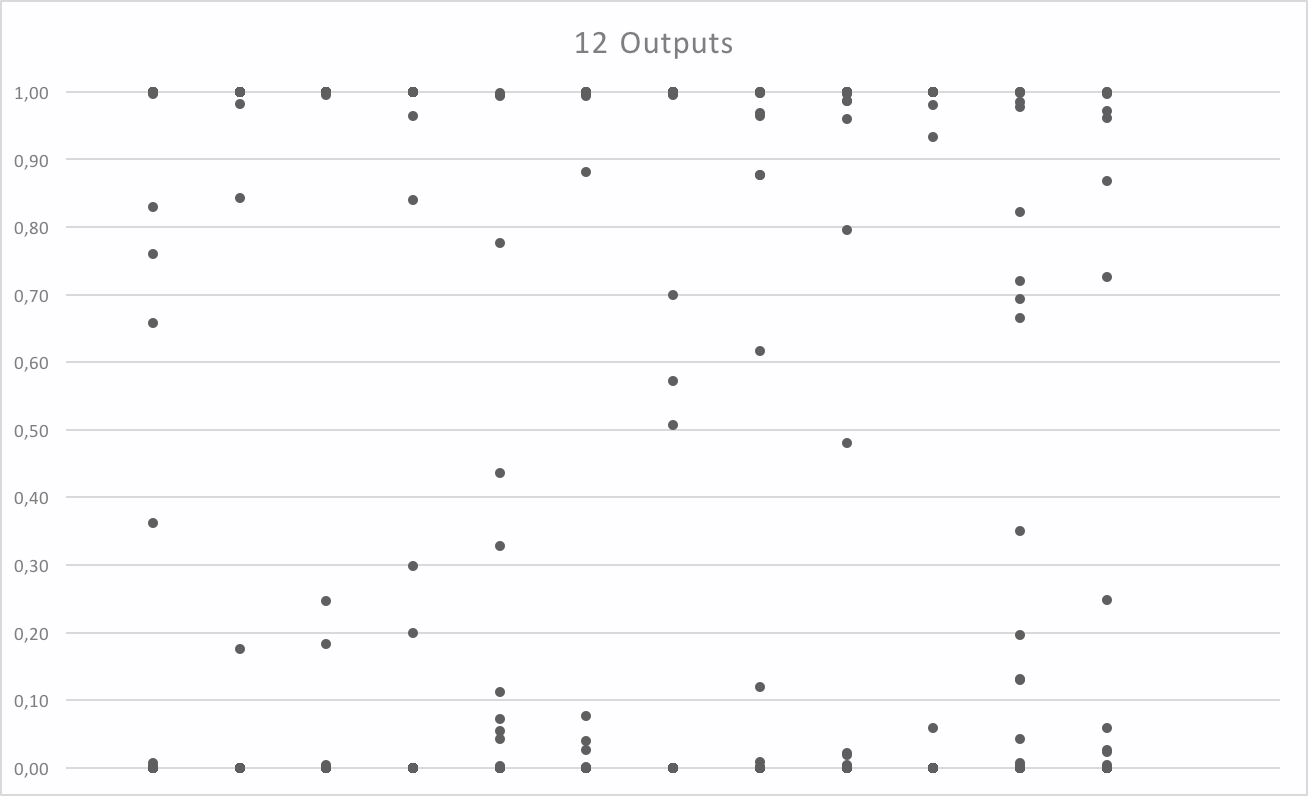
\includegraphics[width=\textwidth]{12_out}
\end{figure}


% Här gör ni en noggrann och neutral beskrivning av iakttagelser och insamlade data från experiment, litteraturstudier och andra typer av undersökningar. Resultaten redovisas på ett sådant sätt att det tydliggörs vad man funnit. Eventuella beräkningar ska också redovisas i denna del. Resultaten behöver bearbetas (struktureras och sorteras) i flera omgångar. Använd gärna tabeller, diagram och grafer för att åskådliggöra dina resultat. Resultatkapitlet ska inte innehålla några tolkningar eller någon diskussion. 

% Gör gärna avslutningsvis en kort sammanfattning av resultaten, särskilt om de är omfattande eller svåra att överblicka för läsaren.  Skriv inte ”mina resultat”, förhåll er neutrala till redovisade data.

% Riktiga toner
\break
\subsubsection{Nätverk 1}


För att testa att lägga in text \\\\\\x.

\begin{centering}
\resizebox{6in}{4in}{
\begin{tabular}{ l | l | l| }
\cline{2-3}
& \multicolumn{2}{c|}{Rätt nod}\\ \hline
\multicolumn{1}{|c|}{\emph{Fall}} & \emph{A4} & \emph{C4} \\ \hline
\multicolumn{1}{|c|}{1}    & 0.530197 & 0.441537 \\ \hline
\multicolumn{1}{|c|}{2}    & 0.528355 & 0.44502 \\ \hline
\multicolumn{1}{|c|}{3}    & 0.528868 & 0.44783 \\ \hline
\multicolumn{1}{|c|}{4}    & 0.528851 & 0.445894 \\ \hline
\multicolumn{1}{|c|}{5}    & 0.524157 & 0.443848 \\ \hline
\multicolumn{1}{|c|}{6}    & 0.533701 & 0.443743 \\ \hline
\multicolumn{1}{|c|}{7}    & 0.522207 & 0.44727 \\ \hline
\multicolumn{1}{|c|}{8}    & 0.530934 & 0.450109 \\ \hline
\multicolumn{1}{|c|}{9}    & 0.530914 & 0.442246 \\ \hline
\multicolumn{1}{|c|}{10}   & 0.525792 & 0.449017 \\ \hline
\multicolumn{1}{|c|}{11}   & 0.52956  & 0.447838 \\ \hline
\multicolumn{1}{|c|}{12}   & 0.528579 & 0.443131 \\ \hline
\multicolumn{1}{|c|}{13}   & 0.52819  & 0.446004 \\ \hline
\multicolumn{1}{|c|}{14}   & 0.528459 & 0.445664 \\ \hline
\multicolumn{1}{|c|}{15}   & 0.526118 & 0.449245 \\ \hline
\multicolumn{1}{|c|}{16}   & 0.529968 & 0.448834 \\ \hline
\multicolumn{1}{|c|}{17}   & 0.527979 & 0.445778 \\ \hline
\multicolumn{1}{|c|}{18}   & 0.528232 & 0.445666 \\ \hline
\multicolumn{1}{|c|}{19}   & 0.528529 & 0.444762 \\ \hline
\multicolumn{1}{|c|}{20}   & 0.527944 & 0.448757 \\ \hline
\multicolumn{1}{|c|}{21}   & 0.530264 & 0.444677 \\ \hline
\multicolumn{1}{|c|}{22}   & 0.526533 & 0.446885 \\ \hline
\multicolumn{1}{|c|}{23}   & 0.529135 & 0.451268 \\ \hline
\multicolumn{1}{|c|}{24}   & 0.527022 & 0.445682 \\ \hline
\multicolumn{1}{|c|}{25}   & 0.529065 & 0.446183 \\ \hline
\multicolumn{1}{|c|}{26}   & 0.526292 & 0.437518 \\ \hline
\multicolumn{1}{|c|}{27}   & 0.532195 & 0.443127 \\ \hline
\multicolumn{1}{|c|}{28}   & 0.523379 & 0.444124 \\ \hline
\multicolumn{1}{|c|}{29}   & 0.532881 & 0.449827 \\ \hline
\multicolumn{1}{|c|}{30}   & 0.523641 & 0.448685 \\ \hline
\multicolumn{1}{|c|}{31}   & 0.532865 & 0.451292 \\ \hline
\multicolumn{1}{|c|}{32}   & 0.523558 & 0.445709 \\ \hline\hline
\multicolumn{1}{|c|}{Medelv.} & 0.528261 & 0.446161\\ \hline
\multicolumn{1}{|c|}{Rätt} & 32 & 0\\ \hline
\multicolumn{1}{|c|}{\%} & 100 & 0 \\ \hline
\end{tabular}

\begin{tabular}{| l | l| }
\hline
\multicolumn{2}{|c|}{Fel nod}\\ \hline
\emph{A4} & \emph{C4} \\ \hline
0,447821 & 0,529853 \\ \hline
0,442688 & 0,525828 \\ \hline
0,452777 & 0,538675 \\ \hline
0,443227 & 0,522045 \\ \hline
0,449508 & 0,530202 \\ \hline
0,44305  & 0,528417 \\ \hline
0,444517 & 0,533847 \\ \hline
0,448503 & 0,522099 \\ \hline
0,446924 & 0,526682 \\ \hline
0,445618 & 0,538008 \\ \hline
0,445414 & 0,516878 \\ \hline
0,447913 & 0,533056 \\ \hline
0,44788  & 0,533912 \\ \hline
0,447484 & 0,522907 \\ \hline
0,444007 & 0,524843 \\ \hline
0,448414 & 0,532862 \\ \hline
0,4445   & 0,532014 \\ \hline
0,450206 & 0,526373 \\ \hline
0,442747 & 0,523086 \\ \hline
0,449423 & 0,538247 \\ \hline
0,446674 & 0,522857 \\ \hline
0,445994 & 0,526291 \\ \hline
0,449005 & 0,525382 \\ \hline
0,443396 & 0,533444 \\ \hline
0,446783 & 0,530342 \\ \hline
0,448209 & 0,525356 \\ \hline
0,443767 & 0,530157 \\ \hline
0,45074  & 0,526417 \\ \hline
0,441478 & 0,53203  \\ \hline
0,450937 & 0,51989  \\ \hline
0,443493 & 0,529569 \\ \hline
0,44967  & 0,527829 \\ \hline\hline
0,446648 & 0,528418 \\ \hline
- & - \\ \hline
- & - \\ \hline
\end{tabular}




% \multicolumn{3}{|c|}{Nätverk 4 med träning $\alpha=0.2$ rätt nod}\\ \hline
\begin{tabular}{| l | l| }
\hline
\multicolumn{2}{|c|}{Rätt nod, $\alpha=0.2$ }\\ \hline
\emph{A4} & \emph{C4} \\ \hline
0.924069  & 0.992079\\ \hline
0.064525  & 0.994155\\ \hline
0.592835  & 0.997007\\ \hline
0.996699  & 0.994699\\ \hline
0.957486  & 0.992996\\ \hline
0.002150  & 0.994996\\ \hline
0.158563  & 0.997109\\ \hline
0.955309  & 0.991146\\ \hline
6.41E-05  & 0.995466\\ \hline
0.999603  & 0.996711\\ \hline
0.9928    & 0.990002\\ \hline
0.989372  & 0.994965\\ \hline
6.12E-05  & 0.997142\\ \hline
0.999558  & 0.993909\\ \hline
0.953059  & 0.989591\\ \hline
0.96366   & 0.99631\\ \hline
0.000111  & 0.998189\\ \hline
0.99906   & 0.984567\\ \hline
0.817736  & 0.992016\\ \hline
0.989201  & 0.997474\\ \hline
0.000644  & 0.994722\\ \hline
0.997747  & 0.989485\\ \hline
0.999029  & 0.99505\\ \hline
0.972834  & 0.9979\\ \hline
0.969881  & 0.993137\\ \hline
0.000300  & 0.990682\\ \hline
0.996966  & 0.99479\\ \hline
0.960684  & 0.995993\\ \hline
0.973331  & 0.996948\\ \hline
0.041084  & 0.993572\\ \hline
0.892258  & 0.991648\\ \hline
0.972593  & 0.995818\\ \hline\hline
0.691664  & 0.994071\\ \hline
23 & 32\\ \hline
71,875 & 100 \\ \hline
\end{tabular}

% }

% \end{centering}

% \multicolumn{3}{|c|}{Nätverk 4 med träning $\alpha=0.2$  fel nod}\\ \hline
% \break
% \resizebox{\textwidth}{!}{
\begin{tabular}{| l | l| }
\hline
\multicolumn{2}{|c|}{Fel nod, $\alpha=0.2$ }\\ \hline
\emph{A4} & \emph{C4} \\ \hline
0,076348 & 0,007774 \\ \hline
0,936125 & 0,005715 \\ \hline
0,416897 & 0,003021 \\ \hline
0,003153 & 0,005171 \\ \hline
0,042617 & 0,006833 \\ \hline
0,997864 & 0,004937 \\ \hline
0,836826 & 0,002880 \\ \hline
0,045434 & 0,008695 \\ \hline
0,999939 & 0,004415 \\ \hline
0,000373 & 0,003310 \\ \hline
0,007243 & 0,009715 \\ \hline
0,010743 & 0,004983 \\ \hline
0,999942 & 0,002873 \\ \hline
0,000418 & 0,005956 \\ \hline
0,046725 & 0,010184 \\ \hline
0,036800 & 0,003698 \\ \hline
0,999892 & 0,001796 \\ \hline
0,000917 & 0,015137 \\ \hline
0,179277 & 0,007792 \\ \hline
0,010877 & 0,002572 \\ \hline
0,999383 & 0,005201 \\ \hline
0,002223 & 0,010286 \\ \hline
0,000933 & 0,004897 \\ \hline
0,027020 & 0,002087 \\ \hline
0,030446 & 0,006786 \\ \hline
0,999712 & 0,009031 \\ \hline
0,003010 & 0,005185 \\ \hline
0,038309 & 0,003936 \\ \hline
0,026727 & 0,003055 \\ \hline
0,959556 & 0,006283 \\ \hline
0,109335 & 0,008270 \\ \hline
0,026621 & 0,004130 \\ \hline\hline
0,308490 & 0,005831  \\ \hline
- & - \\ \hline
- & - \\ \hline
\end{tabular}
}


\end{centering}


\begin{centering}


\resizebox{6in}{3in}{
\begin{tabular}{ |l|l|l|l|l|l|l|l|l|l|l|l|l| }
\hline
% \multicolumn{7}{|c|}{Nätverk 5 med 1 träning $\alpha=0.2$}\\ \hline
\emph{Fall}       & \emph{A\#4 }    & \emph{A4}       & \emph{B4}       & \emph{C\#4 }    & \emph{C4}       & \emph{D\#4} &\emph{D4}       & \emph{E4}        &\emph{F\#4}     & \emph{F4}        & \emph{G\#4}     & \emph{G4} \\ \hline
1 	       & 1.10E-07 & 6.49E-05 & 0.999998 & 1.98E-15 & 0.076692 & 0.037060 &  0.52378  & 1.73E-07  & 0.024735 &  1.54E-13 & 9.67E-13 & 0.83583  \\ \hline              
2 	       & 0.999871 & 1.96E-12 & 0.993727 & 0.999936 & 1.73E-05 & 0.001426 &  2.86E-08 & 0.962536  & 4.63E-07 &  1.06E-15 & 2.96E-10 & 0.99843  \\ \hline              
3 	       & 6.07E-12 & 0.178397 & 4.73E-12 & 9.79E-09 & 1.04E-06 & 6.05E-14 &  3.10E-12 & 9.79E-05  & 0.98278  &  6.01E-15 & 1.81E-06 & 3.77E-08 \\ \hline            
4 	       & 0.999976 & 0.999999 & 1   	    & 6.68E-06 & 3.72E-05 & 0.068889 &  6.78E-14 & 4.93E-08  & 1.42E-10 &  4.55E-05 & 0.121349 & 8.07E-14 \\ \hline              
5 	       & 6.70E-10 & 0.000113 & 0.233541 & 0.999881 & 0.000131 & 0.99947  &  1.38E-13 & 0.009097  & 0.999959 &  1        & 0.977761 & 1.88E-06 \\ \hline        
6 	       & 0.342304 & 1.02E-08 & 7.67E-13 & 4.63E-14 & 0.000120 & 6.34E-17 &  8.71E-10 & 7.94E-05  & 3.39E-11 &  1        & 0.997871 & 0.996374 \\ \hline       
7 	       & 0.000968 & 0.999924 & 1 	    & 0.999986 & 0.000100 & 0.000347 &  0.672319 & 7.67E-10  & 0.999993 &  0.999999 & 0.999214 & 0.676149 \\ \hline                 
8 	       & 0.712442 & 1.00E-12 & 8.68E-09 & 6.52E-16 & 0.003652 & 0.997878 &  0.99987  & 0.001664  & 4.83E-12 &  8.39E-11 & 0.999846 & 2.69E-09 \\ \hline              
9 	       & 3.86E-09 & 1.05E-09 & 2.37E-07 & 0.99997  & 0.000311 & 7.36E-15 &  0.999983 & 0.99934   & 0.999994 &  7.46E-16 & 0.999695 & 5.73E-10 \\ \hline             
10	       & 0.997138 & 1        & 1 	    & 0.30181  & 0.046631 & 7.97E-07 &  0.999962 & 1.23E-09  & 1.03E-12 &  3.41E-15 & 0.966581 & 5.48E-07 \\ \hline              
11	       & 4.55E-07 & 0.999977 & 1.04E-10 & 5.52E-14 & 0.748572 & 0.997839 &  5.49E-06 & 1.77E-12  & 0.999997 &  0.0622781& 0.119313 & 0.004657 \\ \hline                
12	       & 3.45E-05 & 1.95E-14 & 1.38E-07 & 0.999991 & 0.000534 & 1.57E-14 &  4.42E-15 & 0.856928  & 2.28E-12 &  1        & 0.007418 & 0.223541 \\ \hline         
13	       & 0.994893 & 9.91E-10 & 1 	    & 3.26E-16 & 8.68E-06 & 2.03E-06 &  8.09E-16 & 0.999677  & 0.999994 &  1        & 0.001277 & 0.056083 \\ \hline        
14	       & 8.36E-11 & 1        & 2.16E-11 & 0.999975 & 1.29E-06 & 0.999704 &  7.55E-14 & 1.85E-10  & 6.48E-11 &  0.999999 & 0.001192 & 6.08E-08 \\ \hline               
15	       & 0.999464 & 0.999964 & 0.17106  & 0.213922 & 9.80E-08 & 2.26E-16 &  0.537378 & 3.03E-13  & 0.999793 &  8.81E-10 & 0.000393 & 5.02E-09 \\ \hline               
16	       & 8.20E-06 & 1.89E-12 & 1  	    & 5.11E-14 & 1.20E-06 & 0.026365 &  0.999988 & 0.85713   & 1.55E-09 &  2.25E-15 & 0.175147 & 1.97E-06 \\ \hline             
17	       & 6.89E-08 & 5.28E-10 & 1.97E-15 & 0.999991 & 0.118283 & 0.994722 &  0.999965 & 0.997755  & 0.982205 &  6.69E-16 & 0.632919 & 0.023741 \\ \hline              
18	       & 0.621699 & 1        & 1   	    & 5.05E-16 & 0.993417 & 4.12E-15 &  0.995724 & 1.70E-09  & 1.11E-06 &  3.22E-13 & 0.60844  & 0.026152 \\ \hline             
19	       & 0.007744 & 0.999997 & 9.47E-12 & 0.999929 & 0.061301 & 0.849981 &  5.21E-08 & 1.22E-11  & 0.006042 &  0.915432 & 0.774453 & 5.01E-05 \\ \hline                
20	       & 1.71E-09 & 4.86E-11 & 0.000445 & 0.998672 & 3.68E-05 & 1.02E-05 &  1.95E-11 & 0.585034  & 0.763962 &  1        & 0.663805 & 1.27E-06 \\ \hline      
21	       & 0.999973 & 1.18E-13 & 0.99971  & 3.43E-15 & 5.33E-06 & 5.31E-14 &  7.67E-08 & 0.997528  & 1.63E-06 &  1        & 0.311715 & 5.23E-08 \\ \hline      
22	       & 8.79E-12 & 0.999978 & 0.004542 & 0.999991 & 9.84E-08 & 0.990295 &  0.992746 & 5.54E-09  & 0.996798 &  1        & 0.042266 & 8.70E-09 \\ \hline       
23	       & 0.999493 & 1        & 3.52E-09 & 1.05E-12 & 1.01E-06 & 6.95E-10 &  0.995755 & 3.16E-12  & 4.74E-08 &  0.970736 & 0.002689 & 2.16E-05 \\ \hline               
24	       & 3.72E-05 & 0.977592 & 0.999998 & 3.36E-07 & 0.002743 & 4.58E-13 &  8.93E-07 & 0.115062  & 0.995581 &  4.81E-13 & 7.69E-05 & 0.962292 \\ \hline             
25	       & 1.56E-08 & 9.70E-13 & 0.001435 & 0.999892 & 0.998109 & 0.996815 &  6.13E-13 & 0.999339  & 2.82E-08 &  1.93E-15 & 7.60E-07 & 0.948256 \\ \hline             
26	       & 0.999918 & 7.46E-12 & 1.25E-11 & 2.60E-14 & 0.99204  & 2.09E-10 &  6.56E-14 & 3.25E-06  & 0.949045 &  4.71E-15 & 4.14E-09 & 1.62E-09 \\ \hline            
27	       & 1.73E-11 & 0.999946 & 1        & 0.936388 & 0.000330 & 8.84E-14 &  1.60E-09 & 5.94E-13  & 5.55E-07 &  1.65E-13 & 3.50E-11 & 1.89E-12 \\ \hline             
28	       & 0.999937 & 1        & 4.46E-14 & 0.999971 & 8.64E-09 & 0.99933  &  0.998715 & 5.80E-08  & 0.453778 &  2.83E-12 & 8.04E-14 & 7.56E-07 \\ \hline            
29	       & 4.53E-09 & 4.39E-05 & 1        & 1.75E-15 & 9.25E-08 & 2.12E-10 &  0.999987 & 0.999055  & 0.000152 &  7.84E-12 & 8.36E-14 & 0.999899 \\ \hline                
30	       & 0.001101 & 2.18E-12 & 3.98E-09 & 0.999928 & 0.000641 & 4.58E-15 &  0.999986 & 0.958093  & 0.002977 &  3.31E-07 & 3.63E-13 & 0.999439 \\ \hline               
31	       & 0.786122 & 0.8206   & 5.00E-05 & 0.796952 & 0.418373 & 0.999689 &  0.999174 & 7.43E-11  & 0.020662 &  0.999825 & 1.30E-12 & 9.52E-11 \\ \hline             
32	       & 1.20E-07 & 0.999999 & 1        & 7.94E-15 & 0.331436 & 7.59E-09 &  3.25E-09 & 1.43E-11  & 9.00E-06 &  1        & 1.79E-11 & 1.75E-13 \\ \hline\hline      
Medelv.    & 0.358222 & 0.468018 & 0.418890 & 0.476474 & 0.149797 & 0.311244 & 0.4286043 & 0.323075  & 0.380576 &  0.404634 & 0.293857 & 0.242216 \\ \hline  
Rätt & 12       & 15       & 13       & 15       & 4        & 10        	 &  15   & 11        & 12       & 13        & 10       & 8 \\ \hline
\%		   & 37.5     & 46.875   & 40.625   & 46.875   & 12.5     & 31.25    & 46.875    & 34.375    & 37.5     & 40.625    & 31.25    & 25 \\ \hline
\end{tabular}

% }


% \resizebox{6in}{6in}{
% \begin{tabular}{ |l|l|l|l|l|l|l| }

% \hline
% % \multicolumn{7}{|c|}{Nätverk 5 med en träning $\alpha=0.2$}\\ \hline
% &\emph{D4}       & \emph{E4}        &\emph{F\#4}     & \emph{F4}        & \emph{G\#4}     & \emph{G4} \\ \hline
%  0.52378  & 1.73E-07  & 0.024735 &  1.54E-13 & 9.67E-13 & 0.83583  \\ \hline      
%  2.86E-08 & 0.962536  & 4.63E-07 &  1.06E-15 & 2.96E-10 & 0.99843  \\ \hline      
%  3.10E-12 & 9.79E-05  & 0.98278  &  6.01E-15 & 1.81E-06 & 3.77E-08 \\ \hline      
%  6.78E-14 & 4.93E-08  & 1.42E-10 &  4.55E-05 & 0.121349 & 8.07E-14 \\ \hline      
%  1.38E-13 & 0.009097  & 0.999959 &  1        & 0.977761 & 1.88E-06 \\ \hline      
%  8.71E-10 & 7.94E-05  & 3.39E-11 &  1        & 0.997871 & 0.996374 \\ \hline      
%  0.672319 & 7.67E-10  & 0.999993 &  0.999999 & 0.999214 & 0.676149 \\ \hline      
%  0.99987  & 0.001664  & 4.83E-12 &  8.39E-11 & 0.999846 & 2.69E-09 \\ \hline      
%  0.999983 & 0.99934   & 0.999994 &  7.46E-16 & 0.999695 & 5.73E-10 \\ \hline      
%  0.999962 & 1.23E-09  & 1.03E-12 &  3.41E-15 & 0.966581 & 5.48E-07 \\ \hline      
%  5.49E-06 & 1.77E-12  & 0.999997 &  0.0622781& 0.119313 & 0.004657 \\ \hline      
%  4.42E-15 & 0.856928  & 2.28E-12 &  1        & 0.007418 & 0.223541 \\ \hline      
%  8.09E-16 & 0.999677  & 0.999994 &  1        & 0.001277 & 0.056083 \\ \hline      
%  7.55E-14 & 1.85E-10  & 6.48E-11 &  0.999999 & 0.001192 & 6.08E-08 \\ \hline      
%  0.537378 & 3.03E-13  & 0.999793 &  8.81E-10 & 0.000393 & 5.02E-09 \\ \hline      
%  0.999988 & 0.85713   & 1.55E-09 &  2.25E-15 & 0.175147 & 1.97E-06 \\ \hline      
%  0.999965 & 0.997755  & 0.982205 &  6.69E-16 & 0.632919 & 0.023741 \\ \hline      
%  0.995724 & 1.70E-09  & 1.11E-06 &  3.22E-13 & 0.60844  & 0.026152 \\ \hline      
%  5.21E-08 & 1.22E-11  & 0.006042 &  0.915432 & 0.774453 & 5.01E-05 \\ \hline      
%  1.95E-11 & 0.585034  & 0.763962 &  1        & 0.663805 & 1.27E-06 \\ \hline      
%  7.67E-08 & 0.997528  & 1.63E-06 &  1        & 0.311715 & 5.23E-08 \\ \hline      
%  0.992746 & 5.54E-09  & 0.996798 &  1        & 0.042266 & 8.70E-09 \\ \hline      
%  0.995755 & 3.16E-12  & 4.74E-08 &  0.970736 & 0.002689 & 2.16E-05 \\ \hline      
%  8.93E-07 & 0.115062  & 0.995581 &  4.81E-13 & 7.69E-05 & 0.962292 \\ \hline      
%  6.13E-13 & 0.999339  & 2.82E-08 &  1.93E-15 & 7.60E-07 & 0.948256 \\ \hline      
%  6.56E-14 & 3.25E-06  & 0.949045 &  4.71E-15 & 4.14E-09 & 1.62E-09 \\ \hline      
%  1.60E-09 & 5.94E-13  & 5.55E-07 &  1.65E-13 & 3.50E-11 & 1.89E-12 \\ \hline      
%  0.998715 & 5.80E-08  & 0.453778 &  2.83E-12 & 8.04E-14 & 7.56E-07 \\ \hline      
%  0.999987 & 0.999055  & 0.000152 &  7.84E-12 & 8.36E-14 & 0.999899 \\ \hline      
%  0.999986 & 0.958093  & 0.002977 &  3.31E-07 & 3.63E-13 & 0.999439 \\ \hline      
%  0.999174 & 7.43E-11  & 0.020662 &  0.999825 & 1.30E-12 & 9.52E-11 \\ \hline      
%  3.25E-09 & 1.43E-11  & 9.00E-06 &  1        & 1.79E-11 & 1.75E-13 \\ \hline\hline
% 0.4286043 & 0.323075  & 0.380576 &  0.404634 & 0.293857 & 0.242216 \\ \hline  
%     & 11        & 12       & 13        & 10       & 8 \\ \hline
% 46.875    & 34.375    & 37.5     & 40.625    & 31.25    & 25 \\ \hline
% \end{tabular}
}
\end{centering}


\begin{centering}
% Next alpha=0.1
\resizebox{6in}{3in}{
	\begin{tabular}{ |l|l|l|l|l|l|l|l|l|l|l|l|l| }
	\hline
	% \multicolumn{7}{|c|}{Nätverk 5 med 2 träningar $\alpha=0.1$}\\ \hline
	\emph{Fall}       & \emph{A\#4 }    & \emph{A4}       & \emph{B4}       & \emph{C\#4 }    & \emph{C4}       & \emph{D\#4} &  \emph{D4}       & \emph{E4}        &\emph{F\#4}     & \emph{F4}        & \emph{G\#4}     & \emph{G4} \\ \hline
	1 	       & 4.09E-08 & 3.62E-05 & 0.999999 & 2.12E-16 & 0.072891  &  0.0402907     &  0.507793 & 7.40E-08 & 0.022258 & 2.86E-14 & 1.86E-13 & 0.867475 \\ \hline                                                  
	2 	       & 0.999918 & 5.30E-13 & 0.996021 & 0.999984 & 8.44E-06  &  0.00126679    &  6.61E-09 & 0.968369 & 2.16E-07 & 1.76E-16 & 7.09E-11 & 0.998969 \\ \hline                                               
	3 	       & 2.06E-12 & 0.175127 & 1.17E-12 & 1.81E-09 & 4.26E-07  & 1.28E-14       &  5.12E-13 & 6.21E-05 & 0.987159 & 9.85E-16 & 7.59E-07 & 1.51E-08 \\ \hline                                              
	4 	       & 0.999984 & 1        & 1        & 2.60E-06 & 1.98E-05  & 0.0773748      &  1.01E-14 & 1.88E-08 & 4.31E-11 & 2.45E-05 & 0.130196 & 1.73E-14 \\ \hline                               
	5 	       & 2.48E-10 & 6.53E-05 & 0.246453 & 0.999966 & 7.49E-05  & 0.999662       &  2.06E-14 & 0.008100 & 0.999972 & 1        & 0.985411 & 9.81E-07 \\ \hline                                 
	6 	       & 0.361802 & 3.50E-09 & 1.82E-13 & 5.56E-15 & 6.77E-05  & 1.35E-17       &  1.76E-10 & 4.99E-05 & 9.99E-12 & 1        & 0.998749 & 0.997461 \\ \hline                               
	7 	       & 0.000717 & 0.999949 & 1        & 0.999997 & 5.75E-05  & 0.000280676    &  0.699607 & 2.23E-10 & 0.999995 & 1        & 0.999555 & 0.725558 \\ \hline                                   
	8 	       & 0.759771 & 2.57E-13 & 2.92E-09 & 6.98E-17 & 0.0027106 &  0.998624      &  0.999936 & 0.001370 & 1.39E-12 & 2.00E-11 & 0.999917 & 9.02E-10 \\ \hline                                                
	9 	       & 1.46E-09 & 3.83E-10 & 9.76E-08 & 0.999993 & 0.0001884 &  1.56E-15      &  0.999992 & 0.999485 & 0.999996 & 1.27E-16 & 0.999834 & 1.69E-10 \\ \hline                                               
	10	       & 0.997999 & 1        & 1        & 0.29828  & 0.0422539 &  4.13E-07      &  0.999982 & 3.78E-10 & 2.93E-13 & 5.62E-16 & 0.978254 & 2.57E-07 \\ \hline                            
	11	       & 2.26E-07 & 0.999985 & 2.86E-11 & 7.00E-15 & 0.776806  &  0.998602      &  1.56E-06 & 4.14E-13 & 0.999998 & 0.058516 & 0.132103 & 0.004111 \\ \hline                                                  
	12	       & 1.83E-05 & 4.77E-15 & 5.48E-08 & 0.999998 & 0.0003382 &  3.35E-15      &  6.50E-16 & 0.87636  & 6.68E-13 & 1        & 0.006651 & 0.248402 \\ \hline                                      
	13	       & 0.996708 & 3.52E-10 & 1        & 3.53E-17 & 4.31E-06  & 1.13E-06       &  1.23E-16 & 0.99975  & 0.999996 & 1        & 0.000985 & 0.058633 \\ \hline                         
	14	       & 2.87E-11 & 1        & 5.68E-12 & 0.999994 & 5.38E-07  & 0.99981        &  1.14E-14 & 5.24E-11 & 2.13E-11 & 0.999999 & 0.000915 & 2.44E-08 \\ \hline                                         
	15	       & 0.999642 & 0.999977 & 0.182771 & 0.199195 & 3.26E-08  & 4.79E-17       &  0.572193 & 7.01E-14 & 0.999858 & 2.31E-10 & 0.000274 & 1.70E-09 \\ \hline                                             
	16	       & 4.73E-06 & 4.70E-13 & 1        & 6.52E-15 & 4.80E-07  & 0.0270889      &  0.999994 & 0.876898 & 5.79E-10 & 3.80E-16 & 0.196923 & 1.01E-06 \\ \hline                                       
	17	       & 2.85E-08 & 1.78E-10 & 4.40E-16 & 0.999998 & 0.112804  &  0.996541      &  0.999983 & 0.998165 & 0.986522 & 1.10E-16 & 0.693672 & 0.023119 \\ \hline                                              
	18	       & 0.658196 & 1        & 1        & 5.47E-17 & 0.995244  &  8.67E-16      &  0.997352 & 5.34E-10 & 5.71E-07 & 5.79E-14 & 0.665578 & 0.026345 \\ \hline                             
	19	       & 0.007559 & 0.999998 & 2.36E-12 & 0.999982 & 0.0543391 &  0.881046      &  1.07E-08 & 3.07E-12 & 0.004835 & 0.933282 & 0.821565 & 3.30E-05 \\ \hline                                                 
	20	       & 5.89E-10 & 1.30E-11 & 0.000309 & 0.999506 & 2.01E-05  & 6.44E-06       &  3.35E-12 & 0.616402 & 0.79588  & 1        & 0.719606 & 6.38E-07 \\ \hline                               
	21	       & 0.999983 & 3.11E-14 & 0.999838 & 4.11E-16 & 2.53E-06  & 1.12E-14       &  1.96E-08 & 0.998007 & 7.66E-07 & 1        & 0.350764 & 2.06E-08 \\ \hline                            
	22	       & 3.07E-12 & 0.999987 & 0.003684 & 0.999998 & 3.26E-08  & 0.993215       &  0.995406 & 1.86E-09 & 0.997716 & 1        & 0.043027 & 3.05E-09 \\ \hline                                
	23	       & 0.999654 & 1        & 1.12E-09 & 1.26E-13 & 3.94E-07  & 2.35E-10       &  0.997372 & 7.62E-13 & 1.92E-08 & 0.980596 & 0.002212 & 1.35E-05 \\ \hline                                       
	24	       & 2.60E-05 & 0.982619 & 0.999999 & 1.08E-07 & 0.0019326 &  1.01E-13      &  2.57E-07 & 0.12005  & 0.996831 & 9.07E-14 & 4.69E-05 & 0.972111 \\ \hline                                              
	25	       & 5.49E-09 & 2.43E-13 & 0.001052 & 0.999968 & 0.998704  &  0.997844      &  9.16E-14 & 0.999465 & 1.18E-08 & 3.19E-16 & 3.16E-07 & 0.961687 \\ \hline                                                
	26	       & 0.999947 & 2.12E-12 & 3.18E-12 & 3.03E-15 & 0.994199  &  6.55E-11      &  9.72E-15 & 1.64E-06 & 0.959851 & 7.68E-16 & 1.20E-09 & 5.37E-10 \\ \hline                                            
	27	       & 5.95E-12 & 0.999968 & 1        & 0.964372 & 0.0002036 &  1.81E-14      &  3.24E-10 & 1.41E-13 & 2.73E-07 & 2.88E-14 & 7.85E-12 & 4.36E-13 \\ \hline                                          
	28	       & 0.999958 & 1        & 1.01E-14 & 0.999993 & 2.60E-09  & 0.999559       &  0.999319 & 2.37E-08 & 0.480429 & 5.52E-13 & 1.48E-14 & 3.73E-07 \\ \hline                                  
	29	       & 1.81E-09 & 2.31E-05 & 1        & 2.02E-16 & 3.22E-08  & 6.67E-11       &  0.999994 & 0.999246 & 0.000105 & 1.64E-12 & 1.49E-14 & 0.999931 \\ \hline                                           
	30	       & 0.000761 & 5.77E-13 & 1.29E-09 & 0.999981 & 0.0004161 &  8.83E-16      &  0.999993 & 0.963543 & 0.002287 & 1.27E-07 & 6.59E-14 & 0.999639 \\ \hline                                                    
	31	       & 0.829945 & 0.842738 & 2.91E-05 & 0.840568 & 0.436666  &  0.999795      &  0.99953  & 1.96E-11 & 0.019073 & 0.999892 & 2.45E-13 & 2.80E-11 \\ \hline                                         
	32	       & 5.10E-08 & 0.999999 & 1        & 9.49E-16 & 0.32775   &  2.91E-09      &  6.20E-10 & 3.66E-12 & 4.87E-06 & 1        & 3.70E-12 & 3.79E-14 \\ \hline\hline                                    
	Medelv.    & 0.362893 & 0.468764 & 0.419692 & 0.478180 & 0.1505532 & 0.3128439 		&  0.430263996 & 0.325791395 & 0.382899065 & 0.405384677 & 0.303945055 & 0.246359146 \\ \hline
	Rätt & 12       & 15       &  13     & 15        & 4       & 10   			&15		& 11 & 12 & 13 & 10 & 8 \\ \hline
	\%		   & 37.5     & 46.875   &  40.625     & 46.875        & 12.5       & 31.25 &  46.875 & 34.375 & 37.5 & 40.625 & 31.25 & 25 \\ \hline
	\end{tabular}	
% }

% \resizebox{6in}{6in}{
% \begin{tabular}{ |l|l|l|l|l|l| }
% \hline
% % \multicolumn{7}{|c|}{Nätverk 5 med 2 träningar $\alpha=0.1$}\\ \hline
%  \emph{D4}       & \emph{E4}        &\emph{F\#4}     & \emph{F4}        & \emph{G\#4}     & \emph{G4} \\ \hline
%  0.507793 & 7.40E-08 & 0.022258 & 2.86E-14 & 1.86E-13 & 0.867475 \\ \hline                      
%  6.61E-09 & 0.968369 & 2.16E-07 & 1.76E-16 & 7.09E-11 & 0.998969 \\ \hline                      
%  5.12E-13 & 6.21E-05 & 0.987159 & 9.85E-16 & 7.59E-07 & 1.51E-08 \\ \hline                      
%  1.01E-14 & 1.88E-08 & 4.31E-11 & 2.45E-05 & 0.130196 & 1.73E-14 \\ \hline                      
%  2.06E-14 & 0.008100 & 0.999972 & 1        & 0.985411 & 9.81E-07 \\ \hline              
%  1.76E-10 & 4.99E-05 & 9.99E-12 & 1        & 0.998749 & 0.997461 \\ \hline              
%  0.699607 & 2.23E-10 & 0.999995 & 1        & 0.999555 & 0.725558 \\ \hline            
%  0.999936 & 0.001370 & 1.39E-12 & 2.00E-11 & 0.999917 & 9.02E-10 \\ \hline                      
%  0.999992 & 0.999485 & 0.999996 & 1.27E-16 & 0.999834 & 1.69E-10 \\ \hline                   
%  0.999982 & 3.78E-10 & 2.93E-13 & 5.62E-16 & 0.978254 & 2.57E-07 \\ \hline                     
%  1.56E-06 & 4.14E-13 & 0.999998 & 0.058516 & 0.132103 & 0.004111 \\ \hline                      
%  6.50E-16 & 0.87636  & 6.68E-13 & 1        & 0.006651 & 0.248402 \\ \hline              
%  1.23E-16 & 0.99975  & 0.999996 & 1        & 0.000985 & 0.058633 \\ \hline               
%  1.14E-14 & 5.24E-11 & 2.13E-11 & 0.999999 & 0.000915 & 2.44E-08 \\ \hline                        
%  0.572193 & 7.01E-14 & 0.999858 & 2.31E-10 & 0.000274 & 1.70E-09 \\ \hline                       
%  0.999994 & 0.876898 & 5.79E-10 & 3.80E-16 & 0.196923 & 1.01E-06 \\ \hline                    
%  0.999983 & 0.998165 & 0.986522 & 1.10E-16 & 0.693672 & 0.023119 \\ \hline                    
%  0.997352 & 5.34E-10 & 5.71E-07 & 5.79E-14 & 0.665578 & 0.026345 \\ \hline                      
%  1.07E-08 & 3.07E-12 & 0.004835 & 0.933282 & 0.821565 & 3.30E-05 \\ \hline                      
%  3.35E-12 & 0.616402 & 0.79588  & 1        & 0.719606 & 6.38E-07 \\ \hline           
%  1.96E-08 & 0.998007 & 7.66E-07 & 1        & 0.350764 & 2.06E-08 \\ \hline             
%  0.995406 & 1.86E-09 & 0.997716 & 1        & 0.043027 & 3.05E-09 \\ \hline             
%  0.997372 & 7.62E-13 & 1.92E-08 & 0.980596 & 0.002212 & 1.35E-05 \\ \hline                      
%  2.57E-07 & 0.12005  & 0.996831 & 9.07E-14 & 4.69E-05 & 0.972111 \\ \hline                    
%  9.16E-14 & 0.999465 & 1.18E-08 & 3.19E-16 & 3.16E-07 & 0.961687 \\ \hline                      
%  9.72E-15 & 1.64E-06 & 0.959851 & 7.68E-16 & 1.20E-09 & 5.37E-10 \\ \hline                      
%  3.24E-10 & 1.41E-13 & 2.73E-07 & 2.88E-14 & 7.85E-12 & 4.36E-13 \\ \hline                       
%  0.999319 & 2.37E-08 & 0.480429 & 5.52E-13 & 1.48E-14 & 3.73E-07 \\ \hline                     
%  0.999994 & 0.999246 & 0.000105 & 1.64E-12 & 1.49E-14 & 0.999931 \\ \hline                      
%  0.999993 & 0.963543 & 0.002287 & 1.27E-07 & 6.59E-14 & 0.999639 \\ \hline                      
%  0.99953  & 1.96E-11 & 0.019073 & 0.999892 & 2.45E-13 & 2.80E-11 \\ \hline                    
%  6.20E-10 & 3.66E-12 & 4.87E-06 & 1        & 3.70E-12 & 3.79E-14 \\ \hline\hline               
%  0.430263996 & 0.325791395 & 0.382899065 & 0.405384677 & 0.303945055 & 0.246359146 \\ \hline
% 15 & 11 & 12 & 13 & 10 & 8 \\ \hline
%  46.875 & 34.375 & 37.5 & 40.625 & 31.25 & 25 \\ \hline
% \end{tabular}
}

\end{centering}

\begin{center}
\resizebox{2in}{4in}{
\begin{tabular}{|c|c|}
\hline
% \multicolumn{2}{|c|}{Summa av alla resultat från G4. Nätverk 5. 2 träningar}\\ \hline
\emph{Fall} & \emph{G4}\\ \hline
1   & 0.887802 \\ \hline
2   & 1.005143 \\ \hline
3   & 0.034175 \\ \hline
4   & 0.035148 \\ \hline
5   & 0.139851 \\ \hline
6   & 1.008482 \\ \hline
7   & 0.732147 \\ \hline
8   & 0.090149 \\ \hline
9   & 0.301534 \\ \hline
10  & 0.107102 \\ \hline
11  & 0.224261 \\ \hline
12  & 0.260468 \\ \hline
13  & 0.070817 \\ \hline
14  & 0.136160 \\ \hline
15  & 0.097065 \\ \hline
16  & 0.105636 \\ \hline
17  & 0.303373 \\ \hline
18  & 0.048460 \\ \hline
19  & 0.040076 \\ \hline
20  & 0.024852 \\ \hline
21  & 0.218468 \\ \hline
22  & 0.224696 \\ \hline
23  & 0.043835 \\ \hline
24  & 0.982971 \\ \hline
25  & 0.971008 \\ \hline
26  & 0.066624 \\ \hline
27  & 0.103853 \\ \hline
28  & 0.431247 \\ \hline
29  & 1.005932 \\ \hline
30  & 1.005942 \\ \hline
31  & 0.025917 \\ \hline
32  & 0.056114 \\ \hline
\end{tabular}
	
}
\end{center}
\clearpage

\section{DISKUSSION}

\subsection{Tolkning av resultat}

% Resultatdata ska analyseras och därefter tolkas. Analysen ska förenkla. tydliggöra och redogöra för de samband. tendenser och mönster som kan utläsas av de data som finns i resultatkapitlet. Diskutera t ex likheter och avvikelser med referens till egna och andras resultat samt till de teorier som behandlats under 1.2 Teori. Varför blev resultaten som de blev? Vilka variationer eller likheter uppvisas i resultatkapitlet. vilka nya (och oväntade) mönster kan skönjas? 

% Vilka slutsatser kan dras av resultaten. med dess begränsningar. och med hänvisning till tidigare redovisad forskning eller faktalitteratur? Under Slutsatser besvaras samtliga frågeställningar. klart och tydligt, och de ska vara enkla att finna. Om du skrivit en hypotes ska du koppla tillbaka till den i detta avsnitt. Slutsatsen ska vara kärnfull och kortfattad.
\subsubsection{Nätverk 1-3}
Nätverk 1-3 gav mycket dåliga resultat. De var slumpartade och det var omöjligt att dra några andra slutsatser än att ingen av nätverken hade möjlighet att särskilja mellan de olika 87 och 2 tonerna resp. Eftersom att det inte fungerade oberoende av antalet utdatanoder verkar det sannolikt att man behöver ett mycket större antal dolda noder för att det ska vara möjligt att känna igen toner. Då det verkade mer gynnsamt att pröva flera lager gjorde vi det och anpassade koden eftersom att det var osäkert om det överhuvudtaget gick och hur många noder man skulle behöva om man endast hade ett dolt lager.
\subsubsection{Nätverk 4}
{\bf 1.} Sammanställning av mätdata för körning av nätverk 4.\\
{\bf 2.} Sammanställning av mätdata för körning av nätverk 4 tränat en gång med $\alpha=0.2$.\\
\begin{center}
\resizebox{3in}{0.3in}{
\begin{tabular}{c|c|c|c|c|}

\cline{2-5}
& \multicolumn{2}{c|}{{\bf 1}}&\multicolumn{2}{c|}{{\bf 2}} \\ \hline
\multicolumn{1}{|c|}{Ton} & \emph{A4} & \emph{C4}& \emph{A4} & \emph{C4} \\ \hline
\multicolumn{1}{|c|}{Medelv.} & 0.528261 & 0.446161& 0.691664    & 0.994071\\ \hline
\multicolumn{1}{|c|}{Rätt} & 32 & 0 & 23 & 32\\ \hline
\multicolumn{1}{|c|}{\%} & 100 & 0 & 71,875 & 100 \\ \hline
\end{tabular}

}
\end{center}

\paragraph{Inlärning}\hspace{0pt}\\
Den första grafen (2 utdatanoder) visar skillnaden mellan rätt svar och utdatan från noden (1-utdata) under träningen. Man kan tydligt se att felet minskar drastiskt i början och sedan planar ut och stabiliserar sig. Detta är det den bör göra då felet bör vara stort i början och sedan minska när den lär sig. Att den stabiliserat sig innebär med stor sannolikhet att den har hamnat i ett lokalt minimum som mycket väl kan vara det globala. 
\paragraph{Testresultat}\hspace{0pt}\\
Om man jämför före och efter ser man att om vi räknar alla svar över 0.5 som rätt gav noden för A4 alltid rätt svar från början och C4 alltid fel. Trots det att A4 alltid gav rätt svar var medelvärdet nästan samma för dem båda (skiljer sig 0.0821 mellan dem). Om man sedan jämför med efter träning kan man se att antalet rätt för A4 har minskat men säkerheten hos svaren är mycket högre och att medelvärdet har ökat vilket tyder på att nätverket har lärt sig för den tonen. Om man sedan kollar på C4 ser man att den har lärt sig något otroligt med 100\% korrekta svar med en mycket hög säkerhet. Dessutom ger C4 resultat som ligger nära $0$ när A4 ger resultat som ligger nära $1$ och tvärtom. Detta tyder på att nätverket är tränat. Frågan är bara vad det är tränat för det är väldigt intressant att summan av utdatan från de två noderna alltid blir $\approx 1$. Det kan tydas som att nätverket har tränats att svara $1$ om den andra noden svarar $0$. Men eftersom att det gällde både när nätverket var tränat och otränat kan detta inte användas för att säga att det stämmer. Det är fullt möjligt att nätverket kan särskilja de två tonerna A4 och C4 men för att vara helt säker måste fler tester genomföras.
\subsubsection{Nätverk 5}
{\bf1.} Sammanställning av mätdata för körning av nätverk 5 tränat med $\alpha=0.2$.\\
{\bf2.} Sammanställning av mätdata för körning av nätverk 5 tränat ytterligare med $\alpha=0.1$.\\
\begin{center}
\resizebox{6in}{0.3in}{
\begin{tabular}{c|c|c|c|c|c|c|c|c|c|c|c|c| }
\cline{2-13}
&\multicolumn{12}{|c|}{{\bf1}}\\ \hline
\multicolumn{1}{|c|}{Ton} &\emph{A\#4 }    & \emph{A4}       & \emph{B4}       & \emph{C\#4 }    & \emph{C4}       & \emph{D\#4} &  \emph{D4}       & \emph{E4}        &\emph{F\#4}     & \emph{F4}        & \emph{G\#4}     & \emph{G4} \\ \hline
\multicolumn{1}{|c|}{Medelv.}    & 0.358222 & 0.468018 & 0.418890 & 0.476474 & 0.149797 & 0.311244 & 0.428604 & 0.323075  & 0.380576 &  0.404634 & 0.293857 & 0.242216 \\ \hline
\multicolumn{1}{|c|}{Rätt.}& 12       & 15       & 13       & 15       & 4        & 10        	 &  15   & 11        & 12       & 13        & 10       & 8 \\ \hline
\multicolumn{1}{|c|}{\%.}	   & 37.5     & 46.875   & 40.625   & 46.875   & 12.5     & 31.25    & 46.875    & 34.375    & 37.5     & 40.625    & 31.25    & 25 \\ \hline
\end{tabular}
}
\end{center}

\begin{center}
\resizebox{6in}{0.3in}{
\begin{tabular}{c|c|c|c|c|c|c|c|c|c|c|c|c|}
\cline{2-13}
&\multicolumn{12}{|c|}{{\bf2}}\\ \hline
\multicolumn{1}{|c|}{Ton} &\emph{A\#4 }    & \emph{A4}       & \emph{B4}       & \emph{C\#4 }    & \emph{C4}       & \emph{D\#4} &  \emph{D4}       & \emph{E4}        &\emph{F\#4}     & \emph{F4}        & \emph{G\#4}     & \emph{G4} \\ \hline
\multicolumn{1}{|c|}{Medelv.}    & 0.362893 & 0.468764 & 0.419692 & 0.478180 & 0.150553 & 0.312844 &  0.430264 & 0.325791 & 0.382899 & 0.405385 & 0.303945 & 0.246359 \\ \hline
\multicolumn{1}{|c|}{Rätt} & 12       & 15       &  13     & 15        & 4       & 10   			&15		& 11 & 12 & 13 & 10 & 8 \\ \hline
\multicolumn{1}{|c|}{\%	}	   & 37.5     & 46.875   &  40.625     & 46.875        & 12.5       & 31.25 &  46.875 & 34.375 & 37.5 & 40.625 & 31.25 & 25 \\ \hline
\end{tabular}
}
\end{center}

\paragraph{Testresultat}\hspace{0pt}\\
Efter en träning kan man se att nätverket inte svarar över 50\% rätt för någon av tonerna. Man kan också se att medelvärdet av resultaten för varje testfall av respektive ton ligger mycket lågt, i spannet 0.15-0.48. Dessa två faktorer tillsammans innebär att nätverket efter en träningssession inte är kapabelt att särskilja på 12 toner trots att när det svarar rätt är svaret mycket pålitligt, exempelvis ger B4 1 på ett antal toner. 
Om man jämför nätverket efter en träningssession och efter två träningsessioner med avseende på medelvärdet av alla testresultat för t.ex. A\#4 kan man se att det har skett en ökning av medelvärdet även om den procentuellt sätt träffar rätt på exakt lika många toner. Som man kan se i tabellen som är summan av alla resultat när man testade G4 gick summan från Nätverk 5 bara mot 1 när G4 ger rätt svar till skillnad från Nätverk 4 där summan av alla resultat alltid går mot 1. Detta implicerar att Nätverk 4 kan se skillnad på A4 och C4 eftersom att båda dessa nätverk tränas efter samma princip, dock förklarar det inte varför C4 ger $\approx 1$ när A4 ger $\approx 0$ om man spelar en A4 ton. Mer studier och tester måste fortfarande göras.

\subsection{Metodanalys}

De tester som gjorts på de neurala nätverken verkar ha fungerat som de ska då det för säkerhets skulle skrivits ut vilken ton som testats och resultaten skiljer sig mycket vilket är starka bevis för att det gått igenom olika toner och olika sekvenser. Testlistorna består alla av ett antal namn på toner och därefter går nätverket igenom var och en av filerna i motsvarande mapp. Den reservation som finns är att det skulle finnas något fel i koden som missats men det verkar mycket otroligt då koden har bearbetats mycket.\\\par
Ett problem med de tester som gjordes är dock att det är en relativt liten mängd data som testas (32 sekvenser av varje ton). Om man skulle öka antalet inspelade sekvenser kanske man skulle få fram resultat som var mer säkra eftersom att det blir minskar risken av att resultaten påverkas av en ton som var onormal. T.ex. är det fullt tänkbart att orsaken till att A4 i Nätverk 4 gav färre träffar var att de inspelade tonernas kvalité var dålig på grund av något som inte märktes av oss när vi spelade in. \par
Ett problem som dock finns är att bland resulaten räknas det som att nätverket svarat rätt när resultatet för noden som var förväntad att ge det korrekta svaret kommer fram till ett resultat som ligger över $0.5$. Detta innebär att det inte utesluter att det skulle kunna finnas ett resultat från en annan nod som var större än den noden som förväntades ha rätt. 
\\\par
När det kommer till inlärningen skrevs datan ut var 1000:e gång, oberoende av vilken fil som testades. Den gav också endast ut skillnaden mellan önskat svar ($1$) och resultatet för den noden som förväntades ha rätt så eventuellt kan grafen vara något missvisande. Grafen visar inte hur den totala inlärningen gick utan använde endast de olika nodernas inlärningsprocess och använde dessa för att försöka skapa en överblick av inlärningens effektivitet.


\subsection{Bedömning av metodens giltighet}

% Vilka felkällor kan ha haft en större inverkan på resultatet? Vilken påverkan har felkällorna haft? (Eventuella felberäkningar presenteras i resultatdelen.) Vilken giltighet har resultatet?

Det finns ett fåtal problem som kan uppkomma i projektet på grund av hur vi handskas med ljud. 
Men normaliseringen födde nya problem. Ett problem var exempelvis att vi inte visste hur vi skulle normalisera all data. Till en början ville vi normalisera över hela den inspelade datan. Att normalisera med denna metod visade sig vara helt onödigt då vi senare delar upp filen i en massa små filer som var för sig inte var normaliserade. Enbart den absolut högsta toppen i hela filen fick värdet ett. Alla andra toppar kommer ha betydligt lägre värden. Men om vi däremot bestämmer oss för att normalisera över de mindre intervallen vi skär ut så kommer vi få åtminstone få att alla segment vi jobbar med är normaliserade, alltså att alla värden ligger mellan noll och ett. Problemet vi fann med denna metod är att den högsta punkten i intervallet inte nödvändigtvis är en topp på en våg. Detta kan möjligtvis komma att försvåra saker för nätverket. 
Ett annat problem vi kom att tänka på är att var att de inspelade tonerna kommer innefatta svävning medan de genererade inte innefattar det. Vi är osäkra huruvida nätverket påverkades av det. \\ 


En annan felkälla som finns är att NN ibland ger ut olika resultat för samma testfall. Resultaten kan skilja sig och under ($10^{-3}$). Denna skillnad kan ha påverkat nätverkets inlärning om den ger skillnad för samma testfall men eftersom att samma testfall dyker upp flera gånger och att inlärningsfaktorn inte alltid är särskilt stor innebär det att NN har potentialen att rätta de felen som skulle kunna tänkas uppstå. Orsaken bakom felet verkar kunna vara avrundningsfel vid inläsningen från filerna men det förklarar inte varför den avrundar olika från en gång till en annan. Orsaken till att det beter sig oberäkneligt skulle också kunna vara att ett antal av vikterna för nätverken ligger mellan $-1$ och $1$ samtidigt som all data som vi tillhandhåller nätverket ligger inom samma område. Detta kan resultera i att deras produkter ligger väldigt nära noll vilket riskerar att det blir väldigt dålig precision. 

\subsection{Förslag på metodförbättringar}

En sak som skulle kunna förbättra nätverkens inlärning skulle vara att istället för att slumpa en träningslista, slumpa $10^5$ olika testfall och bara undersöka hur väl nätverket svarar när man ger den en lista med data som endast används för att testa nätverken med. 

\subsection{Reflektion över arbetet}


% Det är än så länge för tidigt att säkert säga vad detta arbete har bidragit till men de resultat som vi producerat tyder på att tonigenkänning är ett problem som är för abstrakt att lösa för ett nätverk med ett enda dolt lager om man inte använder ett okänt stort antal med noder i det dolda lagret.
Neurala nätverk är ett väldigt hett forskningsområde och alla sätt som de applicerats bidrar till att utveckla nya metoder och användningsområden. Att kombinera NN med ljud kan mycket väl vara ett ovanligt område men som definitivt bidrar med grundforskning. Genom att visa att identifieringen av ljudkurvor, som in princip är funktioner, är ett abstrakt problem som kräver ett komplext nätverk kan bidra till att man får en annorlunda syn på vad som krävs av ett nätverk som ska lösa en uppgift som ter sig vara mycket mer abstrakt. Men det kan också ge en ny inblick i vad som krävs av oss som konstruktör för att identifiera vad som är ett abstrakt problem eller inte.

% I detta kapitel ställer man sig ”vid sidan om” sitt arbete och betraktar dess resultat och uppläggning. Ni gör här en sorts självvärdering av ert forskningsarbete, rapportera därför arbetets förtjänster och brister. Vad betyder det framtagna resultatet sett mot vad som redan är känt? Vad är nytt och förtjänstfullt? Vad stärker redan befintliga forskningsdata?


\subsection{Framtid}

Något som vore väldigt intressant vore att undersöka hur nätverket reagerar om man ger den toner som den inte alls tränats för att känna igen. Det skulle vara ett intressant försök att se dels hur väl tränat nätverket är och om det går att urskilja likheter mellan tonerna om det ger utslag. Det vore också mycket intressant att försöka använda en rekursiv struktur för nätverket, så kallade rekursiva nätverk, för att se om det blir lättare eller svårare för nätverket att fullföra sina uppgifter. Arbetet öppnar också upp en ny vinkel att analysera nätverken, tränar vi dem att göra det som vi tror? Finns det flera nätverk som kan identifiera toner trots att den är tränad för något helt annat? Möjligheterna som står framför att utveckla och bidra till nya områden är lika många som antalet uppgifter som vi potentiellt kan applicera dessa nya neurala nätverk på.

% Avsluta diskussionskapitlet med att blicka framåt, vilka frågor som fortfarande är obesvarade och vad rapporten kan bidra till i framtiden... 

\newpage



% \bibliography{reference}{}
% \bibliographystyle{unsrt}
\printbibliography

% Ger en titelsida för bilagor
\appendix
\addappheadtotoc
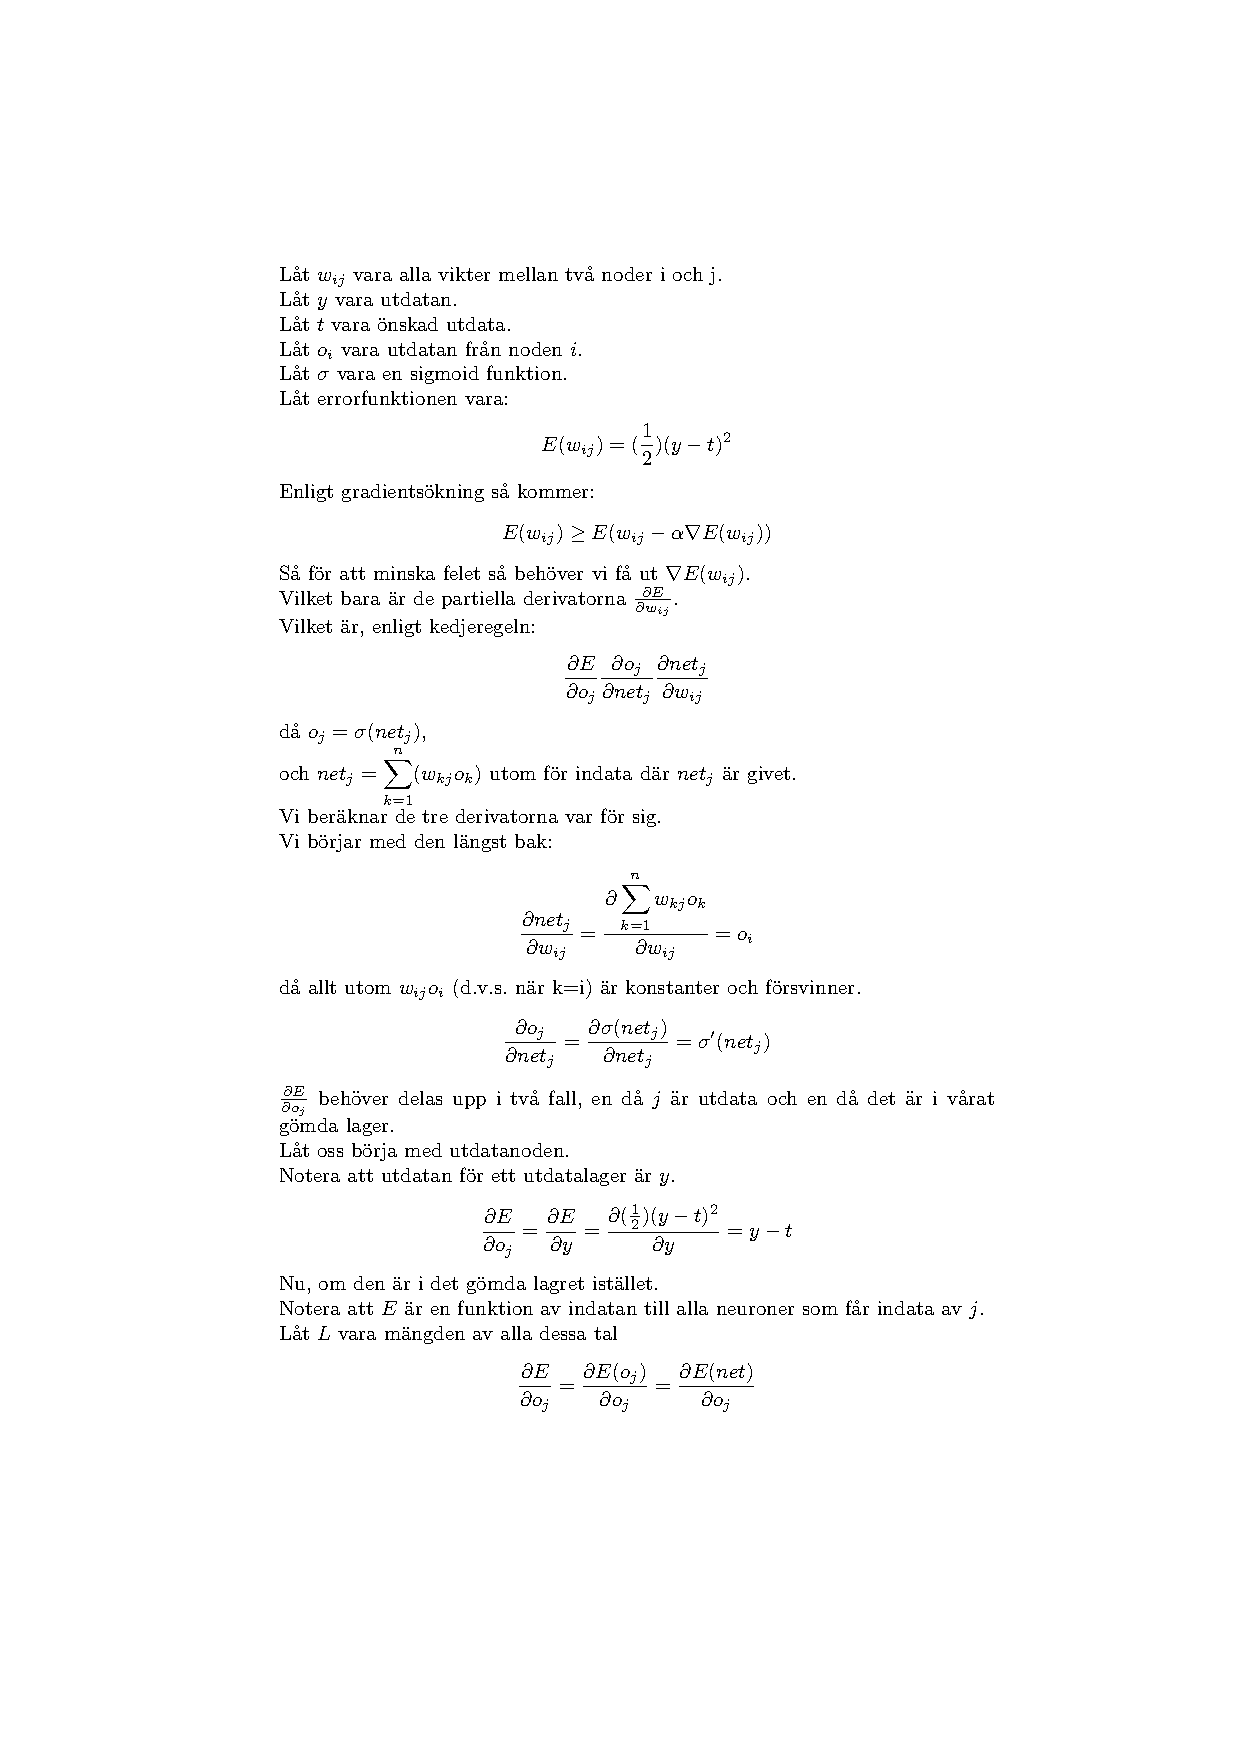
\includepdf[scale=1,pages={1},pagecommand={\section{Backpropagation härledning}\label{BPN}}]{niklas.pdf}
\includepdf[scale=1,pages={2},pagecommand={}]{niklas.pdf}
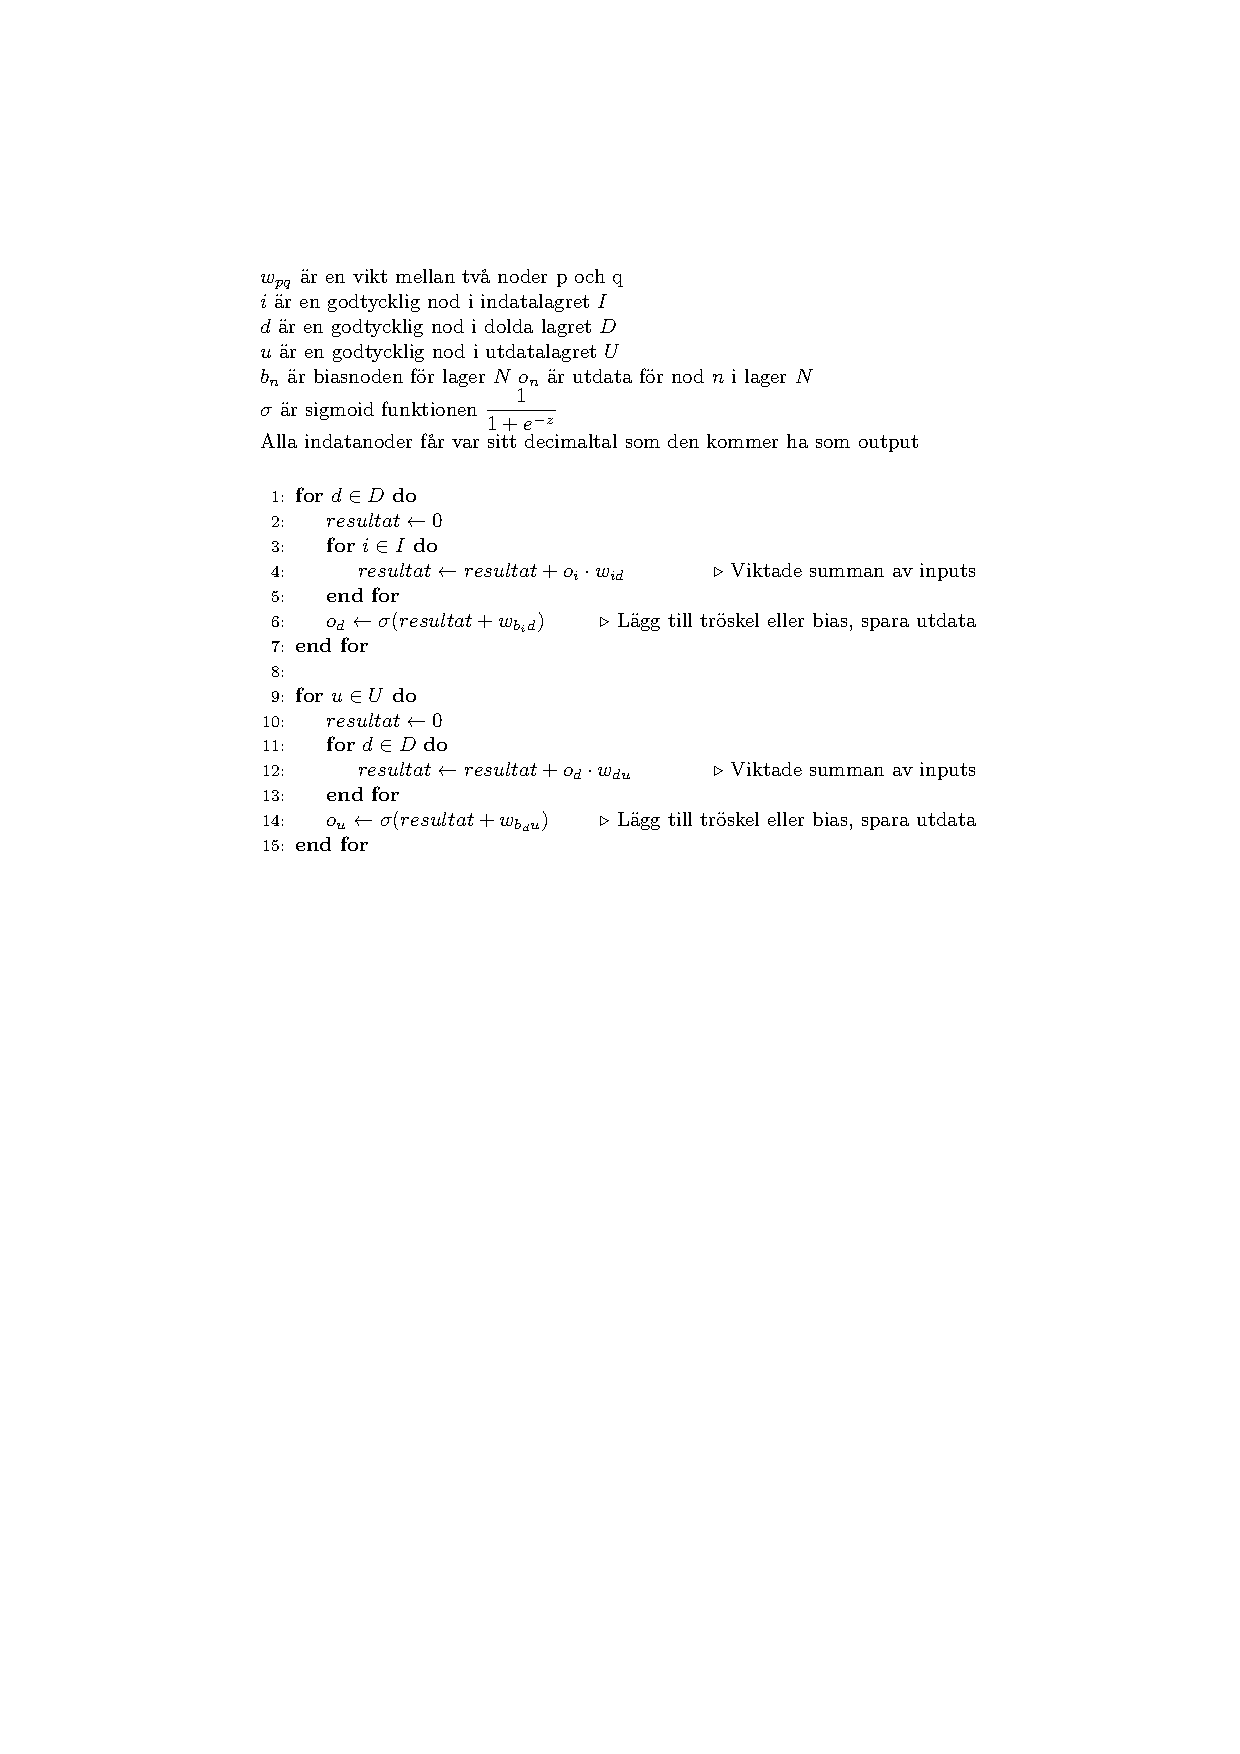
\includepdf[scale=1,pages={1},pagecommand={\section{Pseudokod för körning}\label{Fprop}}]{Fprop.pdf}

\includepdf[scale=1,pages={3},pagecommand={\section{Komplexitet för körning}\label{FPC}}]{BPcomplexitet.pdf}
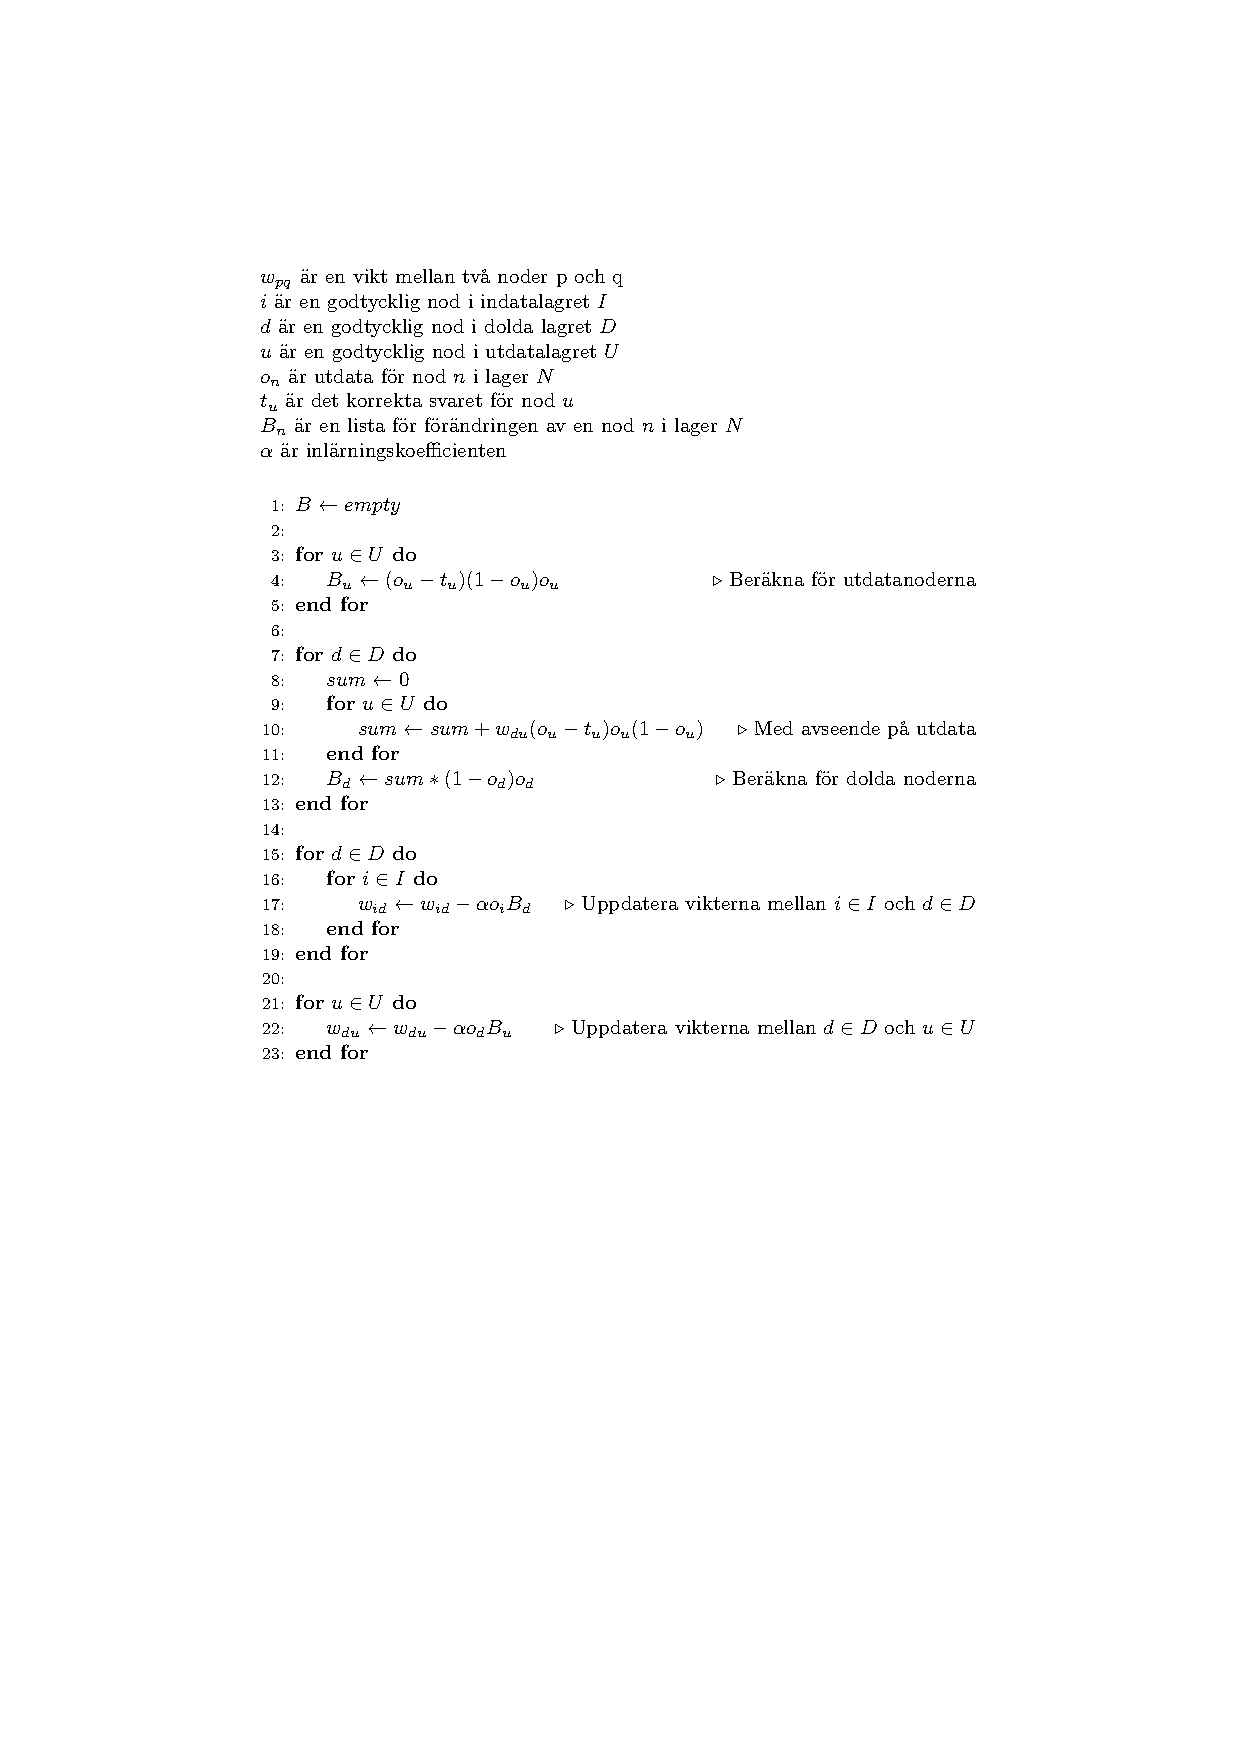
\includepdf[scale=1,pages={1},pagecommand={\section{Pseudokod BP}\label{Pseudo}}]{Pbackpropagation.pdf}

\includepdf[scale=1,pages={2},pagecommand={\section{Komplexitet för BP}\label{BPC}}]{BPcomplexitet.pdf}
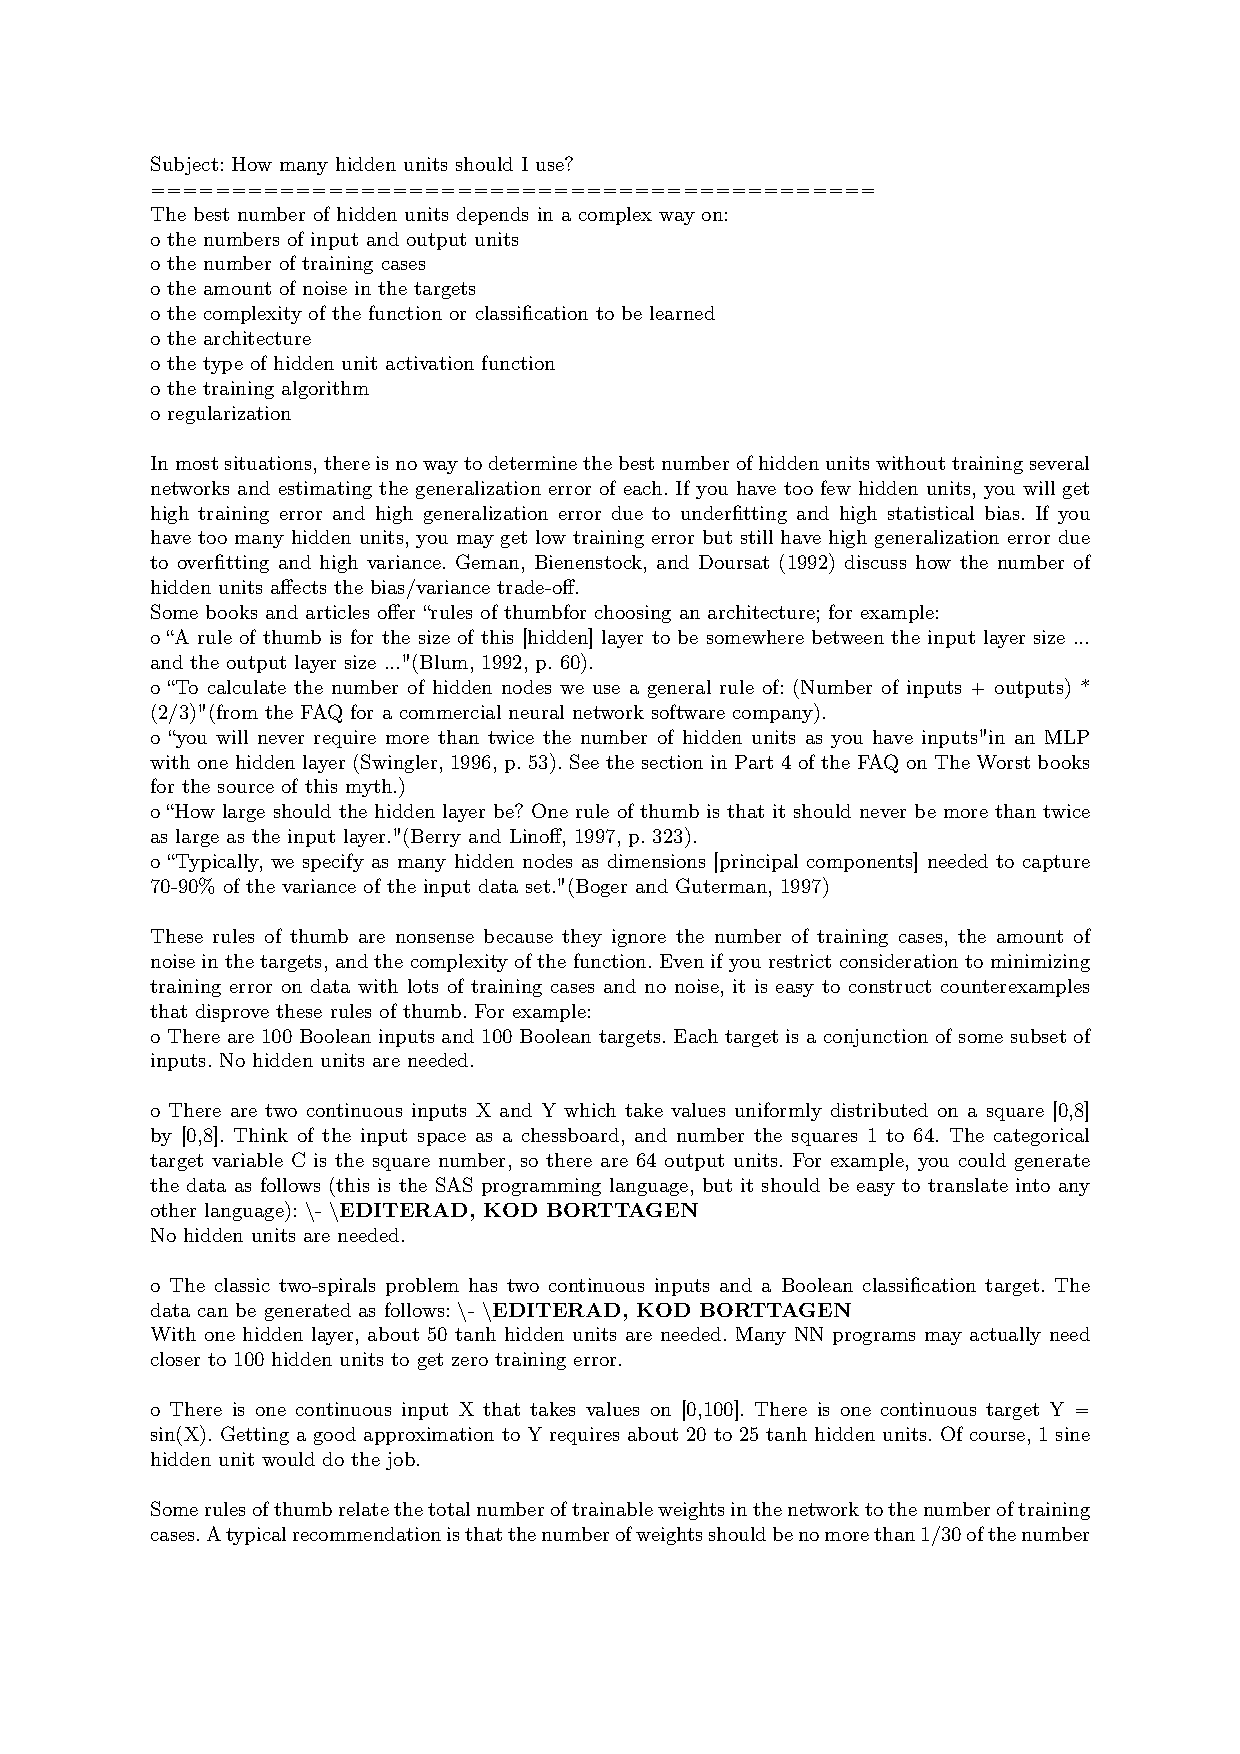
\includepdf[scale=0.95,pages={1},pagecommand={\section{Neural Nets FAQ part 3, utdrag}\label{FAQ}}]{FAQ.pdf}
\includepdf[scale=.95,pages={2-3},pagecommand={}]{FAQ.pdf}




% Ann, K. (2011). Att skriva vetenskapliga rapporter: Anvisningar och rekommendationer för uppsatsskrivande studenter. Stockholm: Stockholms universitet.

% Backman, J. (1998). Rapporter och uppsatser. Lund: Studentlitteratur.

% Chalmers tekniska högskola (2013). Examensarbete. Utformning av rapport. (Hämtad 2013-08-05)

% Dysthe, O., Herzberg, F., Lökensgard Hoel, T. (2002). Skriva för att lära. Lund: Studentlitteratur.

% Engelbertsson, B., & Karlsson, L. (1998). Seminarieuppsatsen: En genomgång av formella krav. Uppsala: Uppsala universitet.

% Holme, I., & Solvang, B. (1997). Forskningsmetodik. Lund: Studentlitteratur.

% Olsson H & Sörensen S (2007). Forskningsprocessen. Kvalitativa och kvantitativa perspektiv. Stockholm: Liber.

% Svenska Språknämnden (2000). Svenska Skrivregler. Stockholm: Liber. 

% BILAGOR

% Enkäter, frågeformulär etc läggs som bilagor. Bilagorna numreras löpande och refereras alltid till inne i den löpande texten, ”se bilaga x”. Om samma referens behöver upprepas skrivs den fortsättningsvis inom parentes, ”(enligt bilaga x)”. 

\end{document}